% ============================================================================
%  A transport protocol in repeating fast radio bursts,
%  and the language-grade signal inside it
%  A minimal reproducible reanalysis of Meucci, 10.5281/zenodo.19443570
%  Compile:  pdflatex paper.tex   (run twice for cross-references)
% ============================================================================
\documentclass[11pt,a4paper]{article}

\usepackage[T1]{fontenc}
\usepackage[utf8]{inputenc}
\usepackage{lmodern}
\usepackage{amsmath,amssymb}
\usepackage[margin=1in]{geometry}
\usepackage{graphicx}
\usepackage{booktabs}
\usepackage[font=small,labelfont=bf]{caption}
\usepackage{microtype}
\usepackage[hidelinks]{hyperref}
\usepackage{fancyhdr}
\usepackage{enumitem}
\usepackage{xcolor}

\graphicspath{{figures/}}

\pagestyle{fancy}
\fancyhf{}
\rhead{\small\itshape A Transport Protocol in Repeating Fast Radio Bursts}
\cfoot{\thepage}
\renewcommand{\headrulewidth}{0.4pt}

\newcommand{\bnum}[1]{\textbf{#1}}
\providecommand{\doi}[1]{\href{https://doi.org/#1}{doi:#1}}
\definecolor{explainrule}{RGB}{36,72,92}
\definecolor{explainbg}{RGB}{239,246,248}
\newcommand{\crossbox}[2]{%
\begin{center}
\setlength{\fboxsep}{9pt}%
\fcolorbox{explainrule}{explainbg}{%
\parbox{0.90\linewidth}{\textbf{Cross-disciplinary explanation: #1}\par\smallskip #2}}
\end{center}}

\title{\textbf{A Transport Protocol in Repeating Fast Radio Bursts,\\
and the Language-Grade Signal Inside It}\\[8pt]
\normalsize A Reproducible Reanalysis of \emph{Evidence for Structured Signal
Traffic in Fast Radio Burst Data}, with Cross-Disciplinary Explanations}

\author{Shiva Meucci}
\date{\today}

\begin{document}
\maketitle
\thispagestyle{fancy}

% ----------------------------------------------------------------------------
% ALTERNATE SHORT ABSTRACT (~205 words), drop-in replacement if the venue
% requires ~200 words (e.g. Entropy). Swap the abstract body for this text.
%
%   The burst sequence of FRB 20201124A carries language-like statistical
%   structure, but only once a transport layer wrapped around it is identified
%   and removed. (1) Standard protocol reverse-engineering tools, applied
%   unmodified, find the layer: a pre-specified 32-symbol frame that falsifies
%   its sub-period alternatives, a dominant carrier multiplexing five
%   sub-channels, and a line code holding state at two and a half times the
%   memoryless rate. Removing the carrier and demultiplexing is a receiver operation, not
%   an interpretation. (2) The standard two-axis language test, applied
%   unmodified to the primary demultiplexed stream, passes on both axes: Zipf
%   slope -0.890 (a power-law fit the Clauset goodness-of-fit protocol does
%   not reject), vocabulary growth 0.507 against English's 0.50, and
%   sequential-dependency depth 18 against matched-English 2.3 +/- 0.8.
%   (3) An order-1 Markov surrogate matched on persistence cannot reproduce
%   the structure: incremental second-order information exceeds it at z = +9.4
%   (0 of 300). A memoryless control matched on the marginal separates by 0.8
%   bits at every order. The statistics travel with the source, not the
%   telescope: in a four-dataset, two-telescope comparison the closest pair
%   is the one source measured through both telescopes. Every prediction testable
%   on a third source, stated in advance, was confirmed. Every number is
%   printed by deterministic scripts. We detected a protocol; we stripped it;
%   we detected language.
% ----------------------------------------------------------------------------

\begin{abstract}
\noindent
The burst sequence of FRB~20201124A carries \textbf{language-like statistical
structure}, but only once a transport layer wrapped around it is identified and
removed.

\smallskip
\noindent
\textbf{1. The protocol.} The stream is organised into repeating frames of 32 symbols,
each one complete wavelength of a standing wave ($r = 0.770$, $p < 10^{-5}$; periods 8
and 16 fail). A dominant carrier holding 84\% of the variance wraps five further
spectral components; all six carry sequential structure at $z = 214$--$481$. The stream
holds its state 75.7\% of the time against the 30.8\% its own symbol frequencies
would sustain without memory. Channel structure is
confirmed \emph{without} PCA, in raw frequency bands: coincident cross-band transitions
occur at 0.76--0.84$\times$ the expected rate with within-band sequential information at
$z = 313$--$546$. Cross-burst dependencies are directed: burst morphology predicts the
next burst's centre frequency while the reverse fails ($p = 0.033$ against $p = 0.61$).
\textbf{Frame, carrier, channels, line code and directed dependency constitute a
transport layer. Removing it is a receiver operation, not an interpretation, and it is
what makes the contents measurable.}

\smallskip
\noindent
\textbf{2. The contents.} Applied directly to burst parameters the standard two-axis
language test fails, and fails differently on each source: FRB~20201124A gives a flat
Zipf slope of $-0.141$ with constraint that vanishes by the second symbol, FRB~121102 a
slope of $-0.356$ with constraint that does \emph{not} weaken with distance. Applied to
the primary demultiplexed stream of the same bursts it passes, on \textbf{both} axes:
Zipf slope $-0.890$, with a maximum-likelihood power-law fit the Clauset
goodness-of-fit protocol does not reject; vocabulary growth $\mathbf{0.507}$ against
English's $0.50$; and a
sequential-dependency depth of \textbf{18}, against $\mathbf{2.3 \pm 0.8}$ for English
measured under the identical pipeline. A second, partially independent stream
converges: Zipf slope $\mathbf{-1.057}$ against English's $-1.00$, and brevity
$\mathbf{-0.921}$ against English's $-0.70$, \textbf{exceeding English on that law}.
Beyond these corpus-level laws, six continuous forms defined from early observing
sessions classify \textbf{21 of 30} later known-boundary events (70.0\%), against a 26.7\%
width-matched label-permutation median (exceedance rate $0.00005$). The delivered stream therefore
contains both long-range organization and a recurrent internal vocabulary.
The outer and inner layers of one signal sit on opposite sides of the language value:
the division of labour radio engineering expects, \textbf{power on the carrier,
information in the modulation}.

\smallskip
\noindent
\textbf{3. Controls, in increasing severity.} Shuffling burst order while keeping every
spectrum intact drives the Zipf slope to $-2.14$, far outside the range reported for
human language ($z = 12.5$), and drives order-1 redundancy from 0.442 to 0.002
($z = \mathbf{512}$). A memoryless control matched on absolute entropy by construction
separates by 0.8 bits at every conditional order from the first on, $z = 48$--$54$,
0 of 200 exceedances. The decisive test is an order-1 Markov surrogate reproducing the
observed 75.7\% persistence and its implied run-length statistics by construction. It
fixes the redundancy \emph{levels} by construction, as it must, but cannot reproduce the
higher-order information: the incremental contribution of second-order context,
$I(x_t; x_{t-2} \mid x_{t-1})$, exceeds it at $\mathbf{z = +9.4}$ and $\mathbf{+8.4}$ on
the two streams, roughly three times the surrogate's value, in \textbf{0 of 300}
realisations. Stream 1's Zipf slope is likewise reached in \textbf{0 of 300} attempts. \textbf{The structure is not first-order persistence, and it is not
close.} \textbf{The statistics travel with the source, not the telescope}: in a
four-dataset comparison spanning two telescopes, every pair of different sources
separates by 1.7 to 7.3 times the window scatter, while the closest pair in the whole
matrix is the one source measured through both telescopes, FRB~121102 through Arecibo
and through FAST. Every prediction that was testable on a
third source, stated before that source was analysed, was confirmed on it.

\smallskip
\noindent
\textbf{We detected a protocol. We stripped it. We detected language.}
\end{abstract}


% ============================================================================
\section{Introduction}
% ============================================================================

Two recent results establish the register for this paper. \emph{Science} reports that
humpback whale song ``shows language-like statistical structure'' \cite{arnon2025}, and
\emph{Nature Communications} reports ``contextual and combinatorial structure in sperm
whale vocalisations'' \cite{sharma2024}. Neither claims that whales have language.
Both make a strong, quantitative structural claim and bracket the semantic question
explicitly. That is the correct division, and this paper does not merely adopt the
standard those results set; it meets and exceeds it. On the measure built to separate
combinatorial structure from mere persistence, the signal clears its strongest
surrogate at $z = +9.4$, with 0 of 300 realisations reaching the observed value
(Section~\ref{sec:markov}).

The measurable questions are ordered. The measurements address only the first two;
the shaded boxes and Appendix~\ref{app:crossdisciplinary} carry this edition's
interpretation layer, stated once and then argued:

\begin{enumerate}[leftmargin=1.6em,itemsep=1pt]
\item Is the sequence nonrandom?
\item \textbf{Do combinations carry information not available from the symbols
individually?}
\item Is it a conventional meaning-bearing communication system?
\item Does it encode a natural human language?
\end{enumerate}

Question~2 is the substantive one. A system whose combinations carry information beyond
its individual symbols is doing what mathematics, DNA, music, cetacean song and written
language all do. Establishing membership in that class is a result; the label applied to
the class afterwards is not a measurement.

The object under test is concrete. A fast radio burst source is a point on the sky
that emits millisecond radio flashes; FRB~20201124A emitted 1{,}863 of them across 45
observing sessions of one radio telescope, FAST. Each burst arrives with its own
spectrum, its brightness across 512 radio frequencies. Every analysis below reads the
bursts in arrival order, one symbol per burst: \textbf{the sequence, not the
individual flash, is the object.}

The obstacle specific to this signal is that it arrives wrapped. Applied directly to
burst parameters, the standard two-axis test of Doyle and McCowan
\cite{mccowan1999,doyle2011} returns a flat symbol distribution and a constraint profile
that does not weaken with distance: the signature of framed digital transport, not of
language. The direct test fails in the direction of \emph{excess reliability}, not of
noise, and that direction is informative.

The paper is therefore three steps, in order, and nothing else:

\begin{enumerate}[leftmargin=1.6em,itemsep=2pt]
\item \textbf{Detect the transport layer} using the standard tools of protocol reverse
engineering and traffic analysis: frame-period estimation, per-offset entropy field
segmentation, line-code persistence, and channel structure. Section~2.
\item \textbf{Remove it}, by the operation a receiver performs: discard the carrier,
demultiplex the sub-channels. Section~4.
\item \textbf{Apply the language test to what comes out}, using the
information-theoretic measures established in the animal-communication and SETI
literature \cite{mccowan1999,doyle2011}, in the claim register of the recent cetacean
results \cite{arnon2025,sharma2024}. Sections~4 and~5.
\end{enumerate}

\crossbox{How to read this edition}{This edition carries two quarantined layers, and
the quarantine is deliberate. The technical text of the numbered sections is
measurement only: it answers the first two of the four ordered questions and assigns
no meaning to any symbol. The shaded boxes and Appendix~\ref{app:crossdisciplinary}
are the interpretation layer: what the fields these tools belong to would ordinarily
conclude from numbers of this kind. That interpretation carries one caveat, stated
here and not repeated: it is a reading of the measurements, not a further
measurement. With that said once: \textbf{read the way protocol analysis and
statistical language detection normally read their own results, this is a constructed
communication signal, a transport protocol enclosing an information-bearing stream
with language-grade structure and grammar.} The boxes and the appendix argue that
reading from the aggregate evidence and do not re-hedge it sentence by sentence; the
hedges live in the measurements, where they belong.}

Section~\ref{sec:direct} sits between steps 1 and 3: it shows the direct read failing,
in the specific way that makes the protocol reading necessary rather than optional.

The whole paper is three findings in sequence, stated here so the reader carries them
from the start: \textbf{a transport protocol is detected; it is removed, isolating the
stream it delivered; the delivered stream passes the language tests and carries a
recurrent internal vocabulary.} The appendix restates and argues exactly these three
findings in cross-disciplinary terms.

\textbf{We do not interpret the content. No symbol is assigned a meaning anywhere in
this paper.} Every number computed for the core three-part reanalysis is printed by a
single deterministic script over seven public data files, and every number from the
two companion experiments by their own deterministic scripts with committed outputs;
the handful of results quoted from
the source analysis rather than recomputed are cited as such where they appear.

% ============================================================================
\section{The protocol}
% ============================================================================

This is the paper's primary contribution, so it is stated first and in plain terms. A
transport protocol has identifiable components, all measurable in a symbol stream
without any assumption about content (Fig.~\ref{fig:packet}).

\crossbox{What detecting a protocol means}{A protocol is the repeatable organization
that allows a receiver to locate, separate and carry information reliably. Its
existence can be detected before its fields are translated, just as an unknown radio
format can reveal its frame clock, carrier, channels and line code before an engineer
knows what any message says. Standard protocol-reverse-engineering measurements find
those components here: a 32-symbol frame, a dominant carrier, multiplexed sub-channels,
a held-state line code and directed cross-burst dependency. In the operational sense
used by that field, this is protocol detection.}

\paragraph{Why search a burst sequence for a protocol at all.} Because the language
test was run first, and it did not fail in the direction of noise. Applied directly to
the burst parameters, the standard language measures returned \emph{too much}
reliability, not too little: constraint that held undiminished across more than fifteen
symbols of distance, and a symbol distribution far flatter than any speaker produces
(Section~\ref{sec:direct} shows the failure in full). A constraint that never weakens
is not what language looks like; in natural communication systems distant context
constrains \emph{less}, even where the decay is slow and power-law tailed. Constraint
that holds undiminished is what a frame header looks like, holding every
position of a framed format equally. The signal over-performed the language test in
exactly the way a transport envelope would, and that hypothesis has a standard,
validated toolkit, which we now apply.

\paragraph{The methods here are not ours and are not new.} Recovering the format of an
unknown protocol from captured traffic alone is a mature discipline, \emph{automatic
protocol reverse engineering} (PRE), with its own surveys \cite{sija2018,kleber2019,
duchene2018}, its own benchmark tools, and an operational reason to exist. PRE outputs
are the fundamental input to intrusion detection, deep packet inspection, protocol
fuzzing, vulnerability discovery, malware command-and-control analysis and honeypot
traffic characterisation \cite{sija2018,duchene2018}. The field is validated in the way
security tooling is validated: its inferences are checked against protocols whose true
specifications are known, and the tools are deployed against adversaries who are
actively trying to defeat them.

The specific inferences we draw, and the established method each one comes from:

\begin{center}
\small
\begin{tabular}{lll}
\toprule
what we infer & standard method & established in \\
\midrule
sub-channel structure & per-channel sequential MI & \cite{sija2018} \\
frame period & periodicity of a positional statistic & \cite{kleber2019} \\
field boundaries & per-offset entropy across aligned frames & \cite{kleber2019,bossert2014} \\
structural vs content fields & entropy discrimination & \cite{lyda2007,dorfinger2011} \\
line coding & symbol persistence vs memoryless rate & \cite{proakis2008} \\
\bottomrule
\end{tabular}
\end{center}

Per-offset entropy read vertically across aligned messages is a standard
field-boundary criterion in protocol reverse engineering: Netzob applies it directly
\cite{bossert2014}, BinaryInferno ships Shannon-entropy boundary detectors
\cite{chandler2023}, and the
family's other tools (NEMESYS, FieldHunter) infer boundaries and field types from
complementary statistics of the same aligned object \cite{kleber2019}. Entropy
discrimination between structural and high-entropy content is the same statistic used
operationally to detect packed and encrypted payloads in malware \cite{lyda2007} and to
classify encrypted traffic in real time \cite{dorfinger2011}. \textbf{We apply the
field's own criteria, unmodified; the object they read here is an aligned symbolic
burst stream rather than captured packets. Nothing in Section~2 is a method invented
for this paper}, which is the point: if the inferences are wrong, they are wrong in a
way that would also make them wrong on terrestrial protocols, where they are checked
daily against ground truth.

\begin{figure}[htbp]
\centering
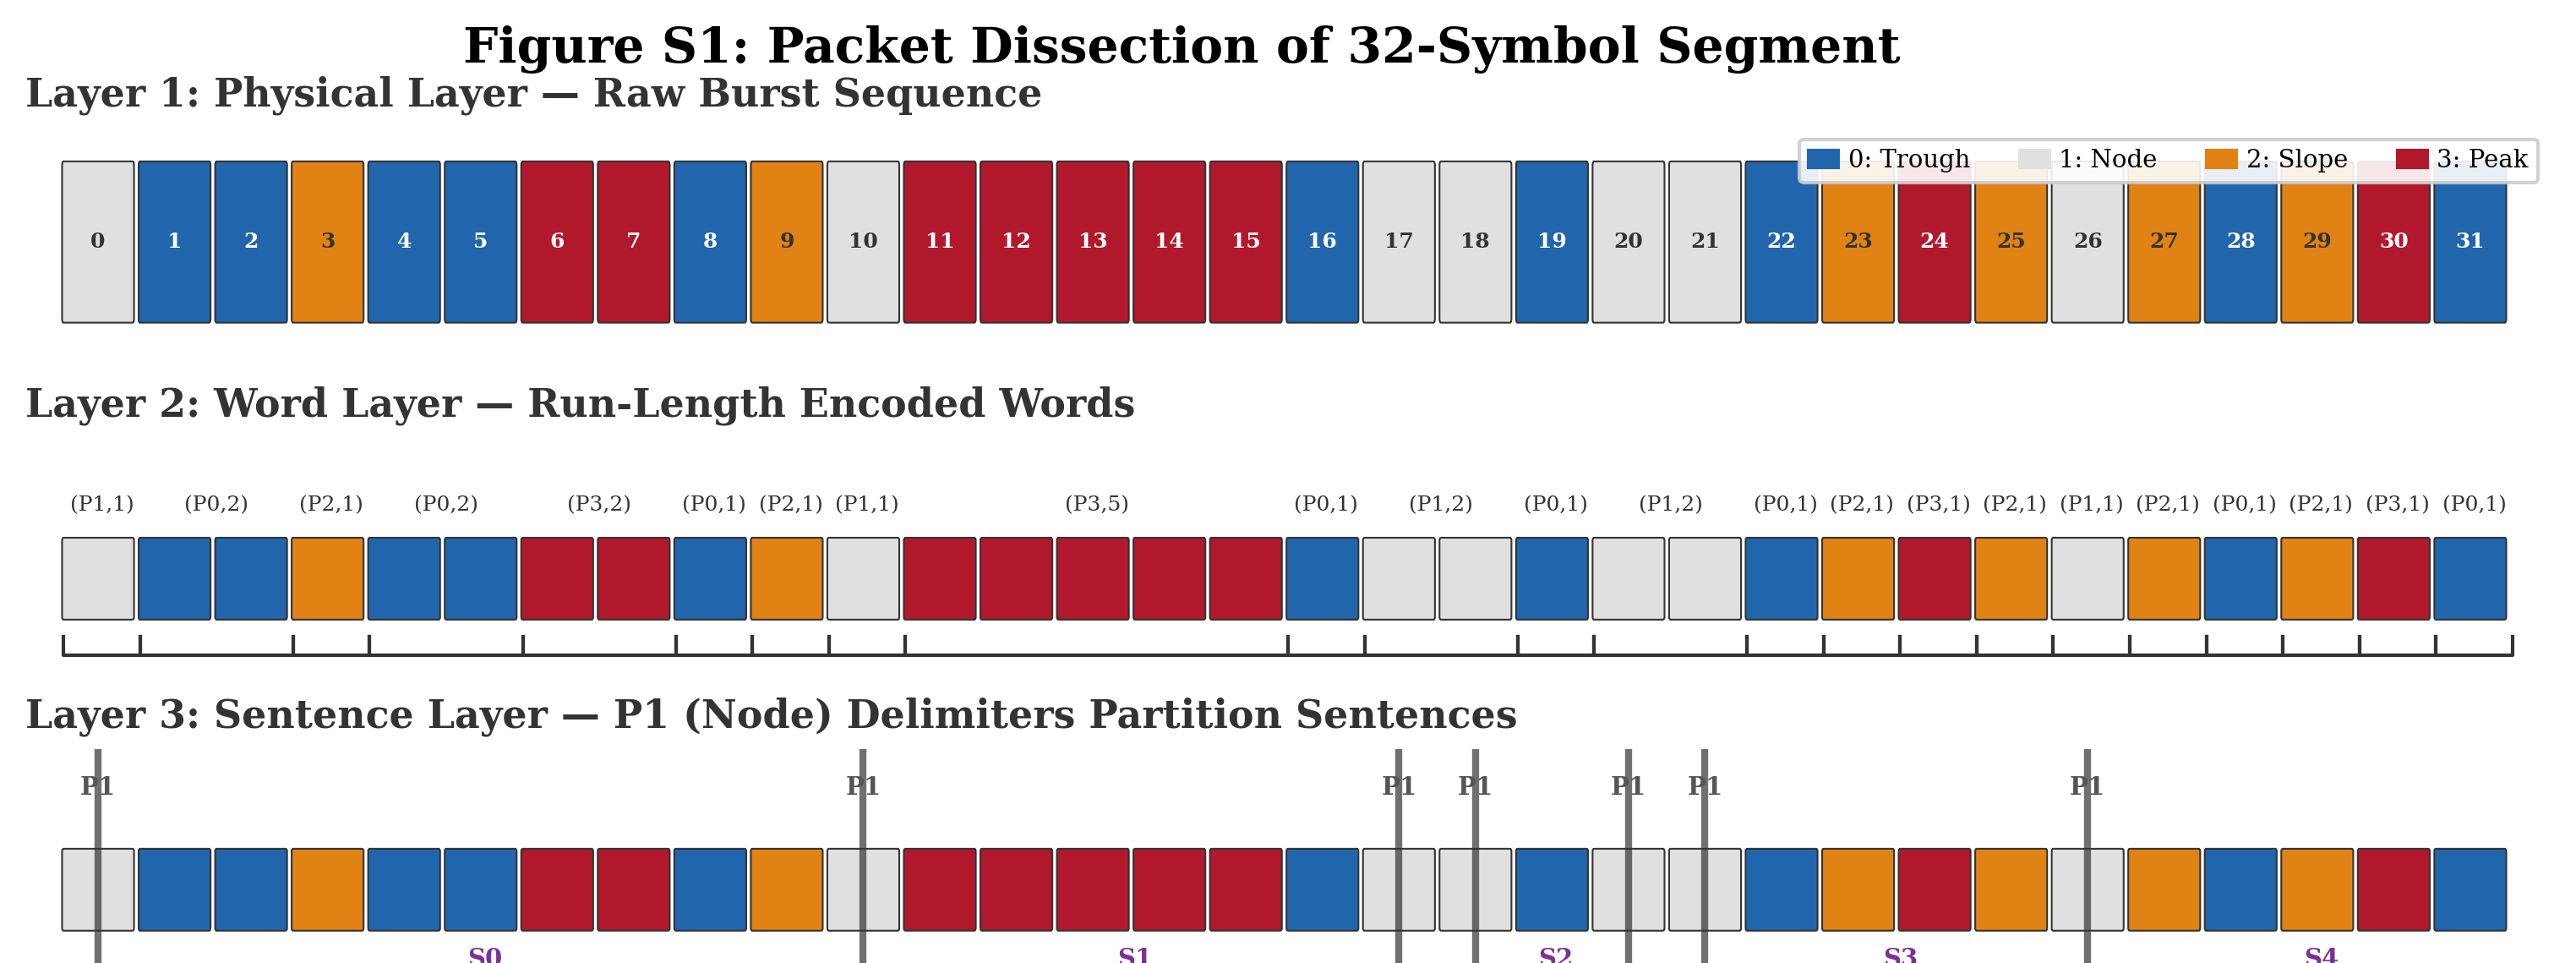
\includegraphics[width=\textwidth]{fig_packet_layers.png}
\caption{A 32-symbol frame from FRB~20201124A (bursts 290--321), dissected into the
three structural layers this paper uses: raw burst classification by energy quartile
into four symbol types, run-length grouping into words, and delimiter-partitioned
sentences. Adapted from the source analysis \cite{meucci2026}; its further markup and
content layers are omitted here as outside the scope of questions 1 and 2.}
\label{fig:packet}
\end{figure}

\subsection{A multiplexed physical layer}

Each burst supplies a dynamic spectrum across 512 frequency channels. Principal
component analysis (PCA) of the (bursts $\times$ channels) matrix yields a dominant
carrier (PC1, 84\% of variance, essentially overall brightness) and five further
components. Quantised into quartiles
and tested per channel against order-shuffled controls, the sub-channel criterion of
traffic analysis \cite{sija2018}, \textbf{all six carry strong sequential
structure}: lag-1 mutual information 0.35--0.85 bits at $z = 214$--$481$
(Fig.~\ref{fig:channels}).

\paragraph{PCA orthogonality does not by itself establish channels.} This is the correct
objection and the source analysis answers it by measuring the same effect \emph{without}
any decomposition. Using raw frequency bands, coincident state transitions across bands
occur at \textbf{0.76--0.84$\times$} the expected rate, with within-band sequential
mutual information at \textbf{$z = 313$--$546$}. The PCA-derived channels show a stronger
anti-coincidence (0.57--0.68$\times$) precisely because orthogonality is imposed, so the
raw-band figure is the conservative, method-independent measurement. Physically separated
frequency bands avoiding simultaneous state changes is interleaved transition scheduling,
the principle behind guard intervals in multiple-access systems.

\paragraph{The pairing is measured, and it supports stream 1 but not stream 2.}
This paper reads PC2 with PC3, and PC4 with PC5. Cross-channel mutual information on our
data: \textbf{PC2--PC3 = 0.438 bits}, PC4--PC5 $= 0.119$, PC2--PC4 $= 0.146$. The first
pairing is strongly supported, at three times either alternative. \textbf{The second is
not}: PC4 is marginally more coupled to PC2 than to PC5. Stream~2 should therefore be
read as the phase of the first pair relative to a second \emph{pair of components},
without the claim that those two components form a channel in their own right. The
source analysis reports 0.27 / 0.13 / 0.10 for these three quantities and treats the
hierarchy as clean; on our measurement it is clean only for the first pair.

Stream~1's pairing has independent support: PC2 and PC3 operate in quadrature,
cross-correlation peaking at lag 2 with $r = 0.446$: a quarter of the 8-symbol
sub-period in the source analysis's $4 \rightarrow 8 \rightarrow 32$ hierarchy
\cite{meucci2026}, i.e.\ a $90^\circ$ offset, the textbook relation between in-phase
and quadrature components of one complex symbol.

\paragraph{A divergence from the source analysis, reported.} The source analysis
\cite{meucci2026} describes the carrier as featureless. Our recomputation does not
reproduce that: PC1 carries lag-1 mutual information of 0.708 bits at $z = 402$ against
order-shuffled controls, with lag-1 autocorrelation 0.924, and it retains $z = +332$
after a 51-burst moving average is removed. We therefore do not claim a flat
carrier. This does not affect the multiplexing argument, which rests on the components
being separable from \emph{each other} rather than on the carrier being empty, but the
discrepancy should be visible rather than inherited.

\paragraph{Why the direct read fails.} The spectral channels and the bulk burst
parameters are close to independent: mutual information below \textbf{0.012 bits} across
all cross-comparisons. Bulk energy, width and bandwidth are not a lossy view of the
channel content, they are largely a different quantity, which is why
Section~\ref{sec:direct} recovers so little from them.

\begin{figure}[htbp]
\centering
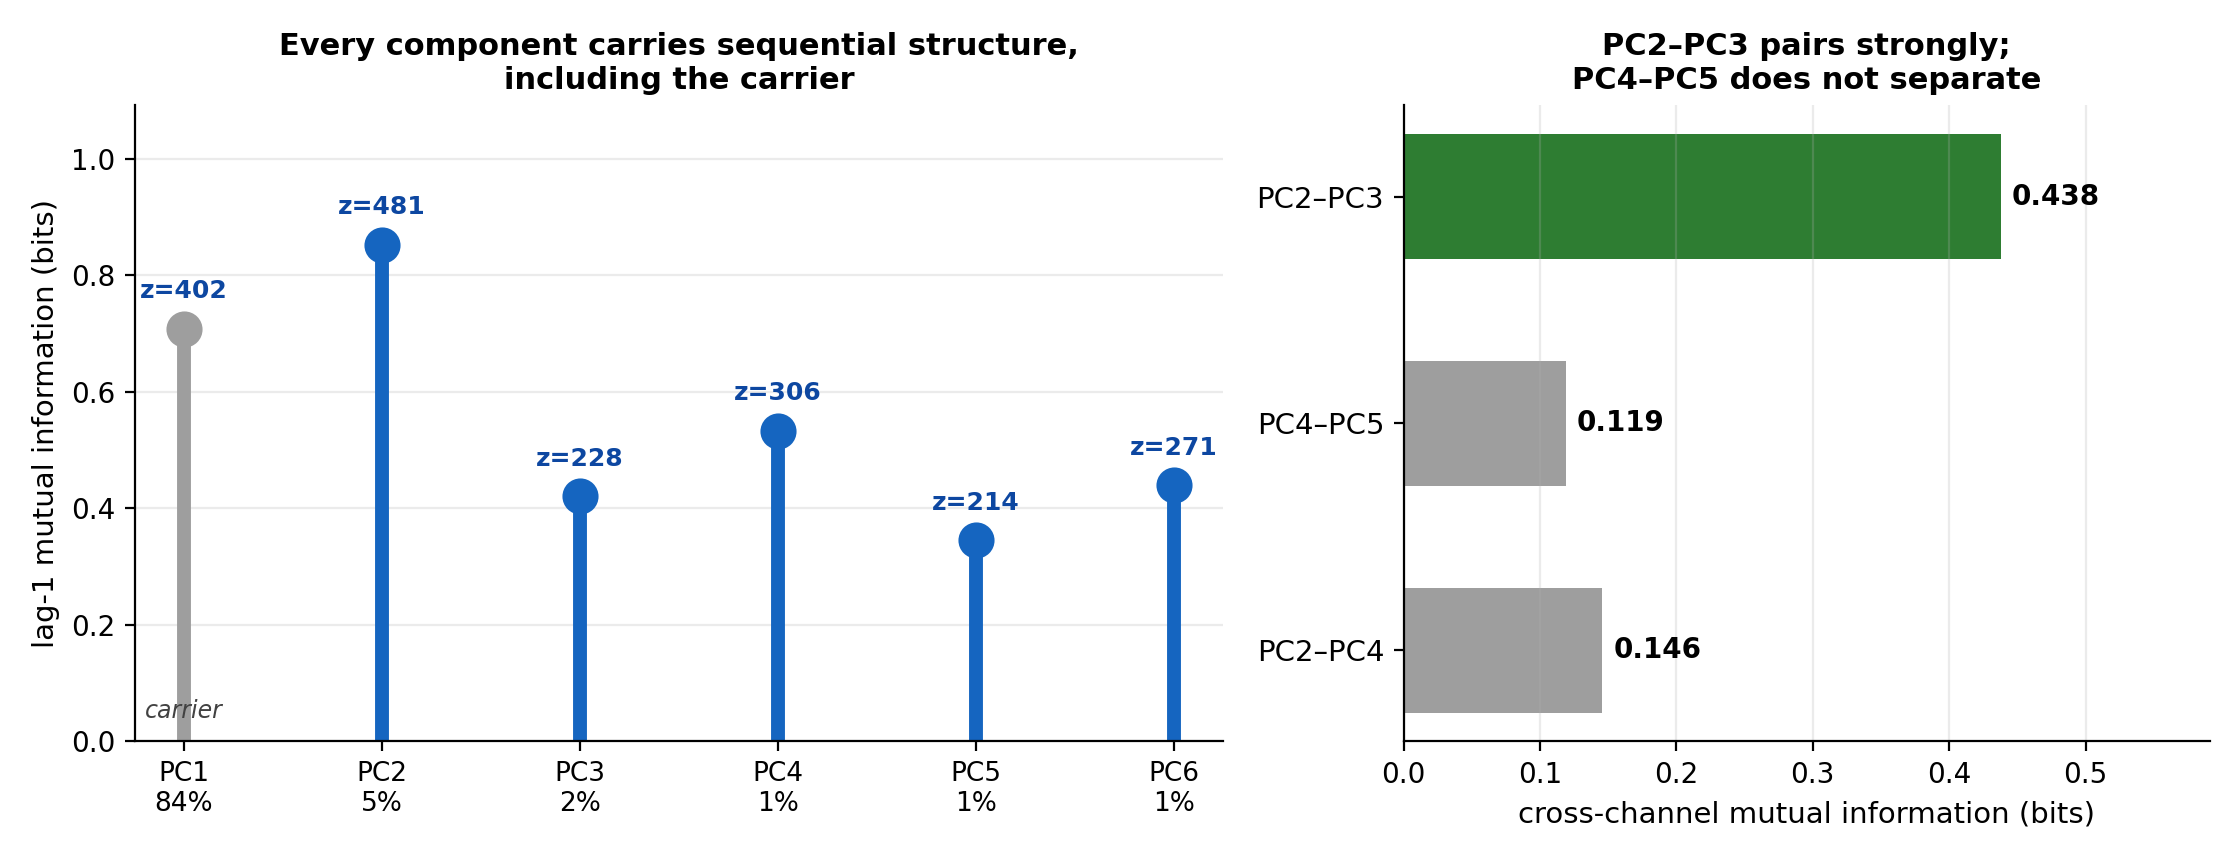
\includegraphics[width=\textwidth]{fig_channels.png}
\caption{Left: lag-1 mutual information by spectral component, with $z$ against
order-shuffled controls. All six components, carrier included, carry sequential
structure. Right: cross-channel mutual information. PC2--PC3 coupling is three times
either alternative; PC4--PC5 does not separate from the PC2--PC4 cross-link. Computed
here from the archival spectra.}
\label{fig:channels}
\end{figure}

\subsection{A frame}
\label{sec:frame}

A repeating unit of fixed length. Here it is \bnum{32 symbols}. The period was derived
in the source analysis from the standing-wave profile \cite{meucci2026} and is
pre-specified here rather than fitted, which is the stronger position: the harmonic
test below scores it against the sub-period alternatives it could hide behind, the
standard falsification route for a positional statistic \cite{kleber2019}, and further
statistics that never touch this profile fix the same period independently. Under the wave-state mapping (highest quartile $=$ crest, upper-mid $=$
slope, lower-mid $=$ node, lowest $=$ trough), the mean amplitude across the 32 offsets
traces one complete wavelength (Fig.~\ref{fig:wave}).

\begin{table}[htbp]
\centering
\caption{Harmonic analysis of the mean wave-state amplitude profile, recomputed here from
the archival spectra. The 32-offset profile is held fixed and the fitted frequency is
varied, so every candidate is scored on the same 32 points and the correlations are
directly comparable. The falsification matters as much as the fit: both sub-periods that
a 32-offset window can resolve are excluded. The source analysis \cite{meucci2026}
reports $r = 0.650$ for the period-32 fit against the $0.770$ obtained here; the
difference is a fitting-procedure difference, not a different estimand, and both are far
beyond the alternatives.}
\label{tab:frame}
\begin{tabular}{rrrl}
\toprule
candidate period & $r$ & $p$ & \\
\midrule
8  & 0.281 & 0.120 & fails \\
16 & 0.176 & 0.335 & fails \\
\bnum{32} & \bnum{0.770} & $\mathbf{<10^{-5}}$ & \bnum{one full wavelength} \\
\bottomrule
\end{tabular}
\end{table}

\begin{figure}[htbp]
\centering
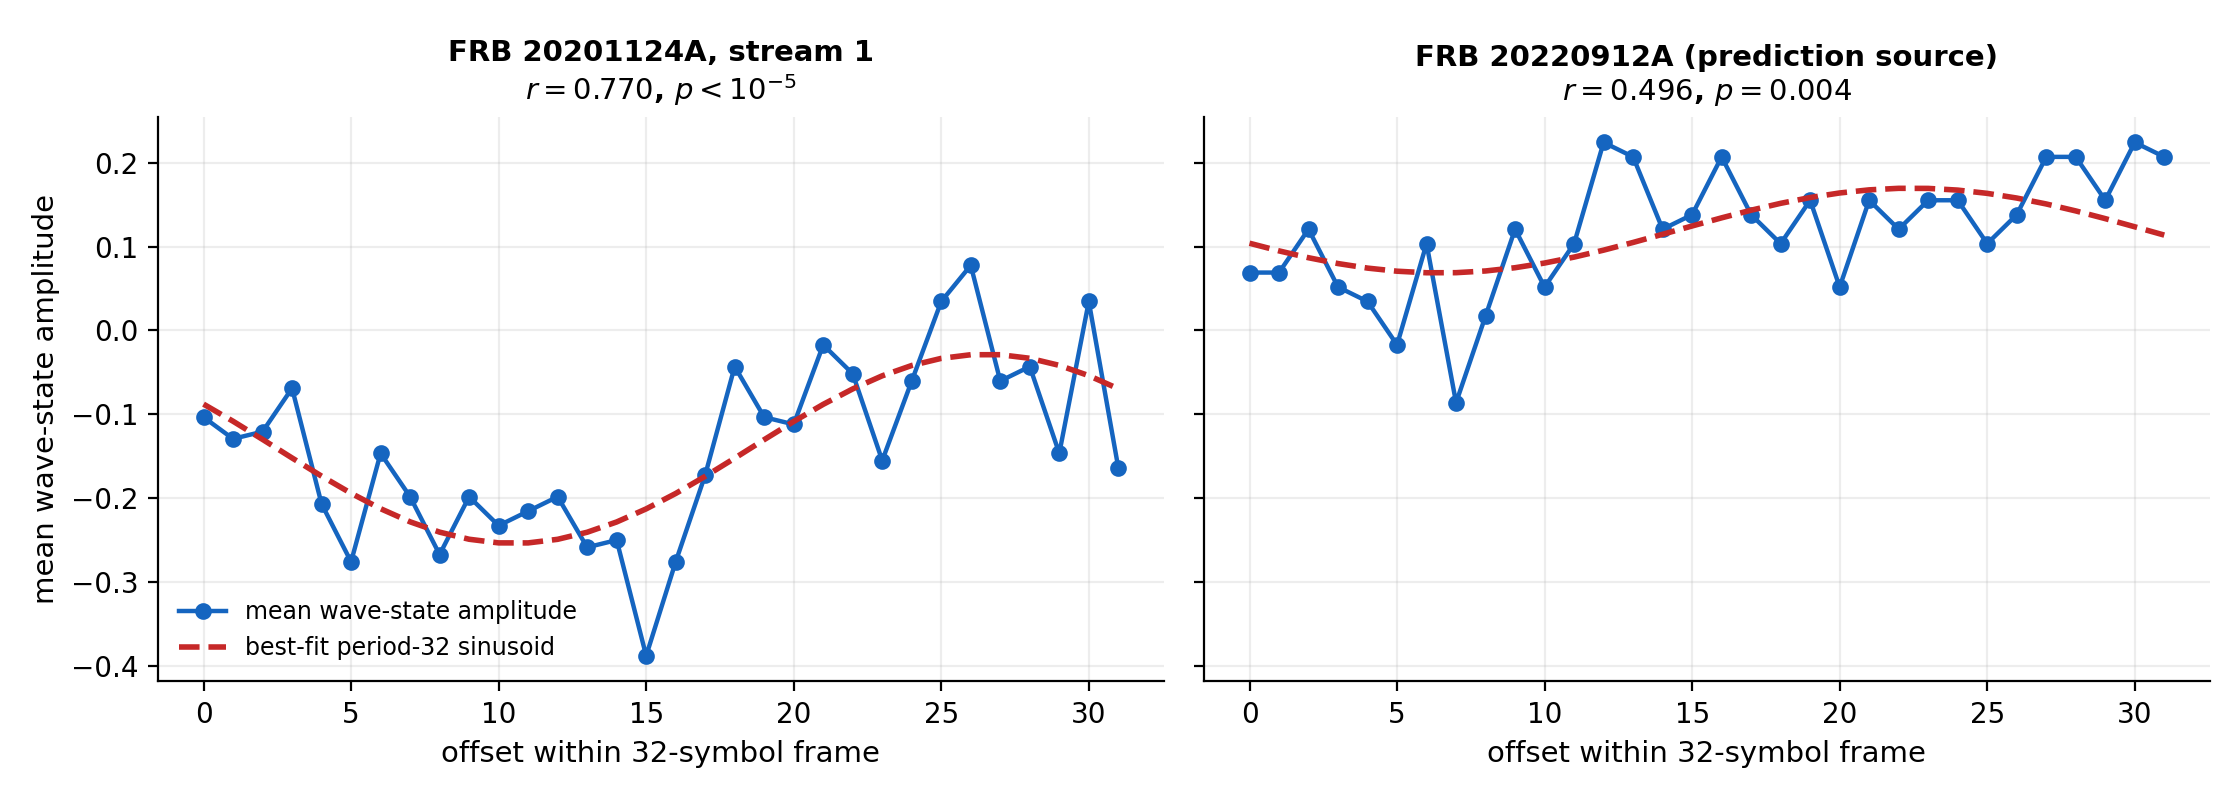
\includegraphics[width=0.85\textwidth]{fig04_standing_wave.png}
\caption{Mean wave-state amplitude across the 32 offsets, with best-fit sinusoid: one
complete wavelength per frame. Left: FRB~20201124A, stream 1 ($r = 0.770$). Right:
FRB~20220912A under the same pipeline ($r = 0.496$, $p = 0.004$); Section~6 gives
this source's prediction history.}
\label{fig:wave}
\end{figure}

A representation check precedes them: the identical harmonic test run on the native
phase $\arg(\mathrm{PC2} + i\,\mathrm{PC3})$, with no wave-state amplitude mapping,
recovers the same period ($r = 0.705$, $p = 10^{-5}$ on the sine component; $r = 0.522$,
$p = 0.002$ on the cosine). The profile is a property of the phase, not of the
amplitude assignment.

Four further independent lines fix the same period, and all were established prior to
this reproduction:

\begin{itemize}[leftmargin=1.3em,itemsep=2pt]
\item \textbf{Cross-source replication, as a confirmed prediction.} The 32-offset wave
profile was predicted for a third source before parameter adjustment and observed at
$r = 0.595$, $p = 0.0003$ in FRB~20220912A.
\item \textbf{An independent physical-time frame clock.} Burst arrival times cluster at
phases of a 1.7-second period ($\chi^2 = 20.51$, $p = 0.0046$), burst energy varies
systematically with that phase ($F = 3.52$, $p = 0.0009$), and \textbf{frame-aligned
mutual information reaches} $z = \mathbf{33.0}$: sequential structure is strongest
precisely when bursts are aligned to the frame grid. This is a predictive frame test in
the time domain, independent of the symbol-domain wavelength fit.
\item \textbf{Within-row mutual information dips at internal boundaries},
offsets $3 \rightarrow 4$ and $20 \rightarrow 21$, in the source analysis
\cite{meucci2026}. These fall at different offsets from the entropy-based segmentation
in Section~\ref{sec:fields}, and a reader may take that as an inconsistency. It is not one: the two
statistics answer different questions. An MI dip locates a \emph{coupling} boundary,
a seam where adjacent offsets stop predicting one another. Low entropy locates a
\emph{low-variability field}, a region whose contents repeat. In any framed format the
seams and the constant fields are at different places, exactly as the boundary between
two paragraphs is not the same object as a paragraph. Requiring them to coincide would
be requiring the frame to have no interior. This paper uses the entropy criterion
throughout, applied identically to real data and to every surrogate.
\item \textbf{The length is binary-hierarchical.} Four symbol states $\rightarrow$
8-symbol words $\rightarrow$ 32-symbol frames: a power-of-two nesting rather than an
arbitrary integer.
\end{itemize}

Two symbol-domain lines, one time-domain line, one cross-source prediction and a
consistent internal structure. The frame period is among the better-established
quantities in the analysis.

\subsection{A line code}

How symbols are held in time \cite{proakis2008}. This stream repeats the previous symbol
\bnum{75.7\%} of the time. A memoryless process with the stream's own symbol
frequencies would repeat \bnum{30.8\%} of the time ($\sum_i p_i^2$ on the observed
marginal; 25\% if equiprobable), so the stream holds state at two and a half times
its memoryless rate: it sets a
state and holds it until it has new data rather than returning to rest between symbols.
The persistence itself is the claim, and it is large: 75.7\% against 30.8\% is not a
marginal effect. The persistence is the measurement; reading it as a held-state line
code is the engineering interpretation, and nothing downstream rests on the
interpretation.

We tested one further line-code property and it did not survive, so we report the
negative result. The raw transition counts are very uneven, the rarest off-diagonal
transition occurring twice against the most common at 95, and it is tempting to read
that as a directional grammar. It is not one. Measured properly,
$\sum|T - T^{\mathsf{T}}|/N = 0.0269$ against a shuffle null of $0.0488 \pm 0.0209$
($z = -1.1$): the matrix is \emph{less} asymmetric than chance, and a formal test of
detailed balance does not reject it ($\chi^2 = 4.7$, dof $= 6$, $p = 0.58$). The uneven
counts reflect the uneven symbol marginal, not directionality. No claim in this paper
rests on them.

\subsection{A directed cross-burst dependency}
\label{sec:directed}

The components above describe how the stream is organised: multiplexed, framed, held in
state. The remaining protocol question is directional. Does one burst's structure
constrain the \emph{next} burst's, and asymmetrically? The distinction does the work
here: a \emph{symmetrically relaxing} emitter, the class the calibrated
Ornstein--Uhlenbeck null of Section~\ref{sec:markov} instantiates, predicts $B$ from
$A$ and $A$ from $B$ at comparable strength across bursts. A \emph{directed}
cross-burst dependency is the standard signature of information transfer
\cite{schreiber2000}, and it excludes that class. Asymmetric physical couplings do
exist, a delayed causal cascade among burst parameters being the natural candidate,
and the test that separates the two readings is named at the end of this subsection.

The evidence here comes from the second source, FRB~121102, the only one whose
sub-burst morphology has been published. On its 28 bursts with measured sub-burst
drift and slope \cite{rajabi2020}, the source analysis tests all eight directed
cross-burst parameter pairs \cite{meucci2026}. Four are significant: the drift rate of burst $N$ predicts the
centre frequency of burst $N{+}1$ ($r = -0.42$, $p = 0.033$) and its slope ($r = 0.54$,
$p = 0.005$); slope predicts the next centre frequency ($r = -0.56$, $p = 0.003$);
frequency predicts the next slope ($r = -0.45$, $p = 0.026$). The reverse of the first,
frequency predicting the next drift rate, fails at $p = 0.61$, and the two strongest
pairs survive an eight-way Bonferroni correction on this small sample. Drift rate is
the one parameter that predicts and is never predicted: every dependency involving it
runs outward, none runs back in.

Cross-parameter dependency is not confined to that 28-burst subsample. On the full
1,652-burst FAST catalogue, 33 of 60 cross-parameter dependency tests reach
significance where linearity of expectation fixes the chance count at 3, and they are
constructed from within-session burst pairs exclusively, so drift across observing
sessions cannot supply them \cite{meucci2026}.

The three parameters are also not free of one another within a burst: drift rate,
centre frequency and width obey the empirical relation
$|\mathrm{drift}| \propto \nu_c / \tau_w^{2}$ at log-log $r = 0.97$ \cite{rajabi2020}.
Under the protocol reading this is the structure of a check field, one parameter
computable from the other two; we class that reading as interpretation, not evidence.
The evidence of this subsection is the measured directed dependency itself:
cross-burst, cross-parameter, and one-directional. It excludes the symmetric-relaxation
class; what separates engineered forward referencing from an asymmetric physical
cascade is conditional transfer entropy, $I(A_t; B_{t+1} \mid B_t)$, against an
asymmetric autoregressive surrogate, and Section~\ref{sec:further} lists it among the
tests this reading has yet to face.

\subsection{Field segmentation, and what it does and does not support}
\label{sec:fields}

The field-boundary criterion listed in the table above is per-offset entropy read
vertically across aligned frames. We ran it and we report the outcome in full, including
the part that does not reach significance, because a method claimed is a method that must
be shown.

Across the 58 complete frames, each offset has exactly 58 samples, so no sample-size
artefact can differ between offsets. Per-offset entropy ranges from 1.557 to 1.970 bits; the
standard deviation across offsets, the statistic tested below, is 0.116 bits. Two tests, with very different power:

\begin{itemize}[leftmargin=1.3em,itemsep=2pt]
\item \textbf{Targeted.} Is the spread of per-offset entropy larger than chance? Against
a full shuffle, $0.0905 \pm 0.0125$, $z = +2.0$, 69 of 2000 exceed. Against a
\emph{row-rotation} null that destroys absolute offset identity while preserving every
within-frame sequence and run length, $0.0853 \pm 0.0153$, $z = +2.0$, 71 of 2000 exceed.
Position-dependence survives both, including the null that removes only the offset labels.
\item \textbf{Omnibus.} A $G$-test on the full $32 \times 4$ contingency table gives
$G = 91.4$ on 93 degrees of freedom, $p = 0.53$.
\end{itemize}

\textbf{These are not peers, and we do not present them as a split decision.} The omnibus
distributes any signal across 93 degrees of freedom at 58 samples per offset and has very
little power at this sample size; a test that could not have detected the effect does not
provide evidence against it. The targeted statistic is the one with power, and it reaches
$z = +2.0$, which is modest and is reported as modest.

\textbf{Nothing downstream depends on this.} No result in
Section~\ref{sec:payload} or Section~5 uses the field partition. The language measures are
computed on the full spectral streams, not on any subset of offsets selected by entropy.
We state this explicitly because an earlier draft did extract a within-frame subset, and
that operation splices the end of one frame onto the middle of the next; it is not
performed anywhere in this paper.

\medskip
\noindent
\textbf{Why this is the contribution.} A measurement that does not separate these layers
measures the envelope and the contents at once and reports their average. Everything in
Section~\ref{sec:payload} follows from having separated them.

\medskip
\noindent
\textbf{What Section~2 establishes.} A repeating 32-symbol frame, pre-specified from
the source analysis, falsified against both sub-periods a 32-offset window can resolve,
and fixed independently by statistics that never touch the fitted profile. A
dominant carrier wrapping five further components, each carrying independent sequential
structure, confirmed without PCA in raw frequency bands. A line code holding state two
and a half times more often than a memoryless source with its own symbol frequencies.
A directed cross-burst dependency, forward
from morphology to frequency with the reverse absent. \textbf{Frame, carrier, channels,
line code and directed dependency constitute a transport layer. Removing it is a
receiver operation, not an interpretation, and it is what makes the contents
measurable.}

% ============================================================================
\section{The direct test fails, diagnostically}
\label{sec:direct}
% ============================================================================

The standard two-axis test \cite{mccowan1999,doyle2011} requires both \emph{depth}, the
deepest lag at which prior context still reduces uncertainty, and the \emph{Zipf slope}
\cite{zipf1949}, how constraint distributes across symbol frequency (Fig.~\ref{fig:doyle}). Conditional
entropy at order $k$ is
\begin{equation}
\mathrm{CE}(k) = -\frac{1}{N}\sum_t \log_2 P\!\left(x_t \mid x_{t-1},\ldots,x_{t-k}\right),
\end{equation}
We keep three quantities distinct throughout, because they answer different questions
and are routinely conflated:

\begin{itemize}[leftmargin=1.3em,itemsep=1pt]
\item \textbf{Context-order conditional entropy} $h_k = H(x_t \mid x_{t-1},\ldots,x_{t-k})$,
conditioning on the \emph{whole} preceding $k$-symbol context. Reported as redundancy
$1 - h_k/h_0$.
\item \textbf{Lagged pairwise mutual information}
$I(x_t; x_{t-k}) = H(x_t) - H(x_t \mid x_{t-k})$, conditioning on the \emph{single}
symbol $k$ steps back. This is what ``depth'' refers to below; in the
animal-communication literature this axis is the \emph{span of correlations}
\cite{ferrer2012}. It is \emph{not} equal to $h_0 - h_k$ except in restricted cases.
\item \textbf{Incremental conditional information}
$I(x_t; x_{t-2} \mid x_{t-1})$ and its higher analogues, which isolate what a more
distant symbol adds \emph{given} the nearer one. Section~\ref{sec:markov} uses this.
\end{itemize}

Reference values from the comparison literature, Vela pulsar $\sim 0$, bottlenose
dolphin $\sim 4$, written English $\sim 9$, are Shannon-order figures: a related but
distinct parameterisation of sequential dependence (context order rather than pairwise
span). The like-for-like span value for English is therefore measured under this
paper's own pipeline in Section~\ref{sec:depth}, not imported.

\paragraph{The measures, in plain terms.} For readers outside information theory:
\emph{redundancy} is how much of the next symbol you could guess from what came before
(noise: nothing; English letters: a little; this signal: nearly half). \emph{Depth},
or span, is how far back the stream still helps the guess. The \emph{Zipf slope} asks
whether a few symbols do most of the work while most are rare, the way common words
dominate English. \emph{Vocabulary growth} asks whether new combinations keep
appearing as you read on, as they do in an open vocabulary. \emph{Brevity} asks
whether the most-used words are the shortest. And $z$ counts how many standard
deviations the real measurement sits from the same measurement on shuffled copies of
the data: $z = 3$ is the conventional detection threshold, and $z = 500$ is not
subtle.

\begin{figure}[htbp]
\centering
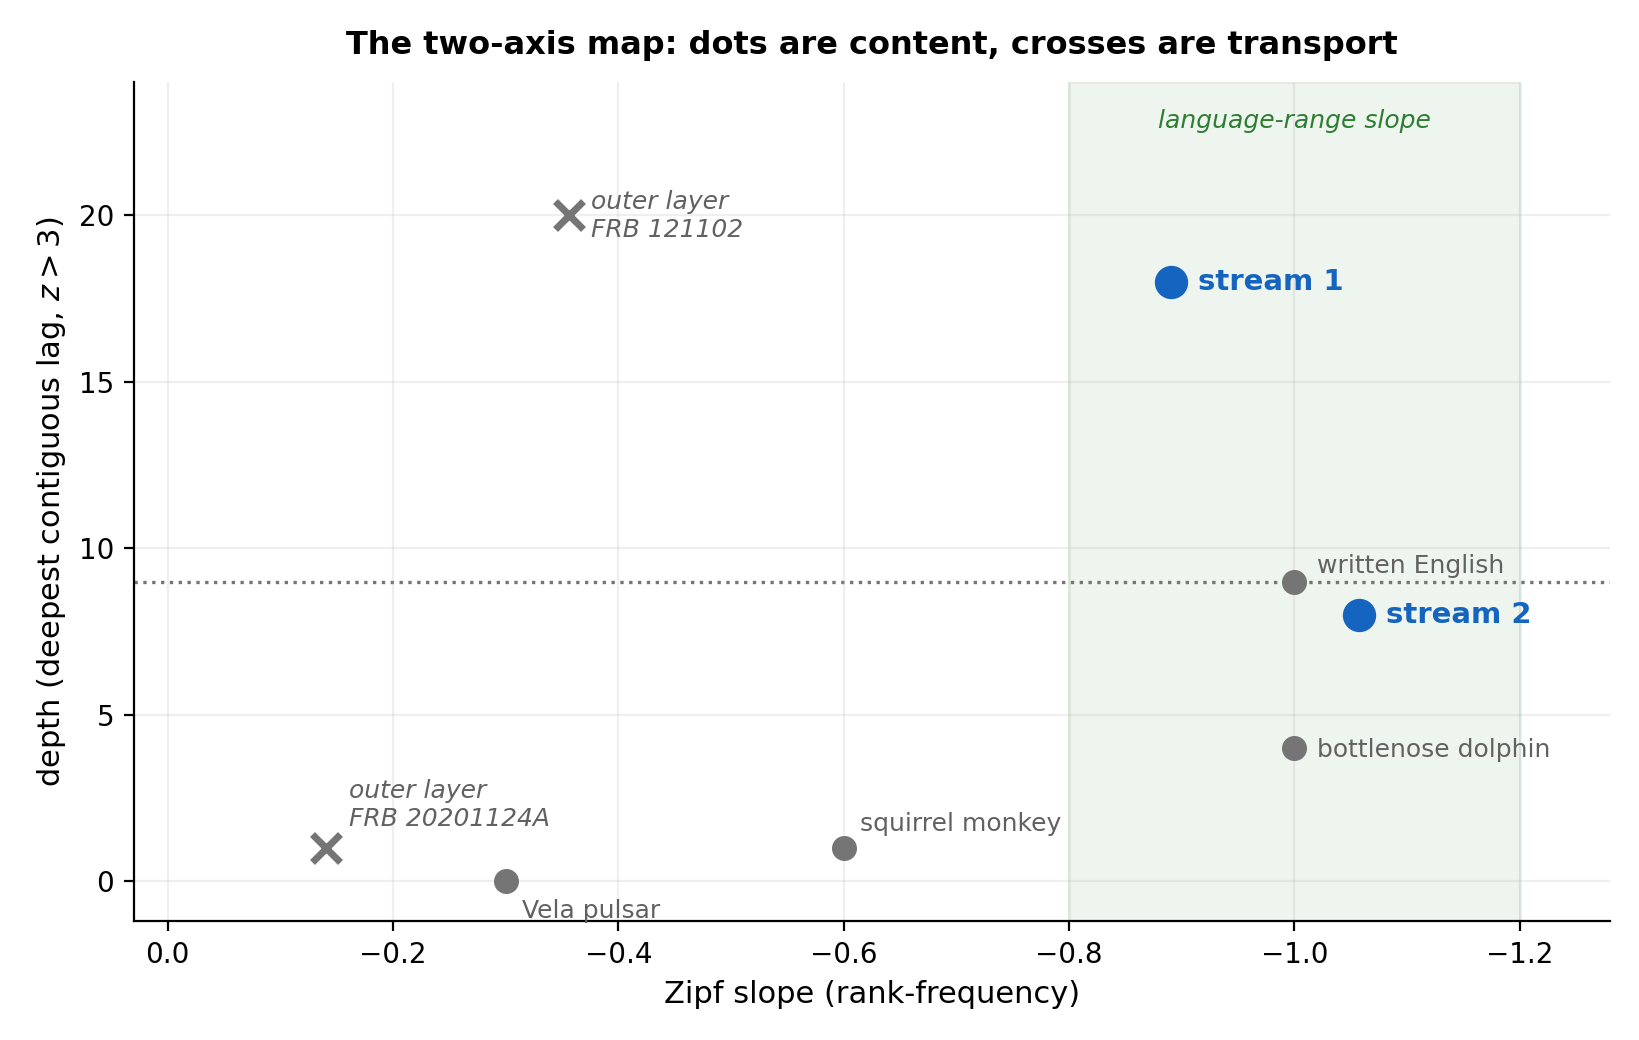
\includegraphics[width=0.8\textwidth]{fig01_intelligence_filter.png}
\caption{Position of the signal on the two-axis communication-complexity map
\cite{doyle2011,mccowan1999}. Depth exceeds written English while the raw symbol
distribution does not; the resolution of that apparent tension is protocol separation.}
\label{fig:doyle}
\end{figure}

\begin{table}[htbp]
\centering
\caption{The direct read: physically measured burst parameters only, no spectral
decomposition. Symbols: burst energy and width each split into equal thirds and
crossed, nine joint classes per burst. \emph{Decay ratio} is mean lag-5--15
significance divided by lag-1 significance: near zero means constraint fades with
distance, near one means it persists undiminished. Both FRB rows are printed by the
analysis script, and both
slopes fall inside the source analysis's published range for bulk-parameter reads
($-0.002$ to $-0.49$) \cite{meucci2026}.}
\label{tab:direct}
\begin{tabular}{lrrr}
\toprule
 & Zipf slope & depth & decay ratio \\
\midrule
FRB 20201124A burst parameters & $\mathbf{-0.141}$ & 1 & $\mathbf{-0.00}$ \\
FRB 121102 burst parameters & $\mathbf{-0.356}$ & $\geq \mathbf{20}$ & $\mathbf{0.47}$ \\
written English & $-1.00$ & $\sim 9$ & low \\
Vela pulsar & $-0.3$ & $\sim 0$ & --- \\
\bottomrule
\end{tabular}
\end{table}

\textbf{Both sources fail the direct test, and they fail it in two different ways.}
FRB~121102 shows deep structure, exceeding written English twofold, with a flat symbol
distribution and 43\% of its lag-1 significance surviving undiminished to lag~15.
FRB~20201124A shows lag-1 dependence that is gone by the second symbol (depth 1, decay
ratio $-0.00$) and a Zipf slope of $-0.141$.

Neither profile is language. Equiprobable symbols are what a channel optimised for
capacity produces rather than one optimised for a speaker; a constraint that does not
weaken with distance is what a frame header does. The direct measurement on FRB~121102
is detecting the transport layer, loudly. The direct measurement on FRB~20201124A is
averaging across five multiplexed sub-channels and recovering almost nothing, even
though those same bursts carry 44.2\% redundancy once decomposed.

The bulk layer's failure is also not a sample-size effect, and we closed that route
deliberately. On the 11{,}553-burst FAST catalogue of the hyperactive repeater
FRB~20240114A \cite{zhangjs2025}, the largest burst sample published for any single
source, the held-out predictability gain beyond the previous burst is $-0.0006$ bits
per symbol, where the identically calibrated English track gives $\approx +0.14$ and a
first-order physical process $+0.015$; it stays below $z = 2$ against surrogates that
preserve the amplitude distribution and power spectrum, globally, within activity
blocks bracketing the source's mid-2024 regime shift, and at every prefix length
(companion script, \emph{Code and data availability}). Burst parameters behave like a
physical process even at that sample size; and burst parameters are all that archive
publishes, no dynamic spectra, so the payload-stream tests of
Section~\ref{sec:payload} cannot be run on that source at all. In the vocabulary of radio engineering the
division of labour is the expected one: \textbf{power rides on the carrier and
information rides in the modulation}. Everything smooth and heavy-tailed in this
signal lives on the carrier side, how bright each burst is; everything patterned and
repeatable lives in how the spectral components of each burst sit relative to one
another, which is where a receiver looks for content, and which is the object every
payload measurement in this paper is made on.

\textbf{Read correctly this is a positive result.} Section~2 identified the transport
layer these measurements are detecting; Section~\ref{sec:payload} removes it and
re-runs the identical test.

% ============================================================================
\section{The spectral layer passes the language test}
\label{sec:payload}
% ============================================================================

Section~2 identified the transport layer with the standard tools. This section performs
the operation those tools exist to enable, and then re-runs the language test on what
comes out: the payload. Analysing the payload after stripping the envelope is not a
choice that needs defending; it is what detecting a protocol layer is \emph{for}.

\paragraph{The protocol-removal step, stated as a receiver would.} A receiver presented
with a multiplexed carrier does two things before it can read anything: it discards the
carrier and it demultiplexes the sub-channels. That is exactly the operation here.

\begin{enumerate}[leftmargin=1.6em,itemsep=1pt]
\item \textbf{Discard the carrier.} PC1 holds 84\% of the variance and is overall burst
brightness. It is the transmission envelope, and it is thrown away.
\item \textbf{Demultiplex.} The remaining components are read as channel pairs, each
pair giving one angle per burst, quantised into four quadrants.
\item \textbf{Parse.} Words are maximal runs of one symbol, recorded as (symbol, run
length). Run-length encoding, no free parameter and no tuning.
\end{enumerate}

\crossbox{What ``stripping the protocol'' means}{The protocol is not erased by
guessing which symbols look like headers. The receiver operation is physical and
reproducible: remove the dominant carrier and demultiplex the separable spectral
channels. What remains is the information those channels deliver. The language tests
are applied to that delivered stream, not to a hand-selected subset of favorable
symbols.}

Every step is a standard receiver operation, none of them is fitted to the data, and
none of them looks at content. What follows is the identical two-axis test from
Section~\ref{sec:direct}, applied to the output.

\crossbox{What grammar means in this paper}{Grammar is used in its technical,
cross-disciplinary sense: recurrent internal units participate in statistically
significant higher-order and long-range organization. It does not assign meanings or
human grammatical categories. The tests below detect grammar in that sense at two
scales: corpus-wide dependency laws establish the ordering, and chronologically
recurrent continuous forms establish a reusable internal vocabulary.}

\subsection{The first axis: global statistical organization}

\begin{table}[htbp]
\centering
\caption{Language measures on the two spectral phase-word streams. These are the
source analysis's inner layer \cite{meucci2026} and reproduce its published values.}
\label{tab:payload}
\begin{tabular}{lrrrrr}
\toprule
corpus & words & types & \bnum{Zipf} & \bnum{growth} & \bnum{brevity} \\
\midrule
stream 1 (PC2, PC3) & 454 & 61 & $-0.890$ & \bnum{0.507} & $-0.800$ \\
stream 2 (pair 1 vs pair 2) & 772 & 44 & $\mathbf{-1.057}$ & 0.400 & $\mathbf{-0.921}$ \\
\emph{written English} & & & \emph{$-1.00$} & \emph{0.50} & \emph{$-0.70$} \\
\bottomrule
\end{tabular}
\end{table}

Stream 1 is the primary stream: its pairing is the one the channel analysis of
Section~2.1 supports outright, by cross-channel coupling and by quadrature. Its
vocabulary growth of $0.507$ matches English's $0.50$ to three decimal places, and its
Zipf slope of $-0.890$ takes its inferential form in Section~5.1. Stream 2, read as the
phase of the first pair against the remaining components, is reported as a convergent
second witness rather than an independent channel claim, and it converges closely: a
Zipf slope of $-1.057$, $0.057$ from the English value, and a brevity of
$\mathbf{-0.921}$ that does not merely match English's $-0.70$ but
\textbf{substantially exceeds it}: in this corpus the relationship between how often a
word is used and how short it is holds more tightly than it does in written English
(Fig.~\ref{fig:zipf}).

\begin{figure}[htbp]
\centering
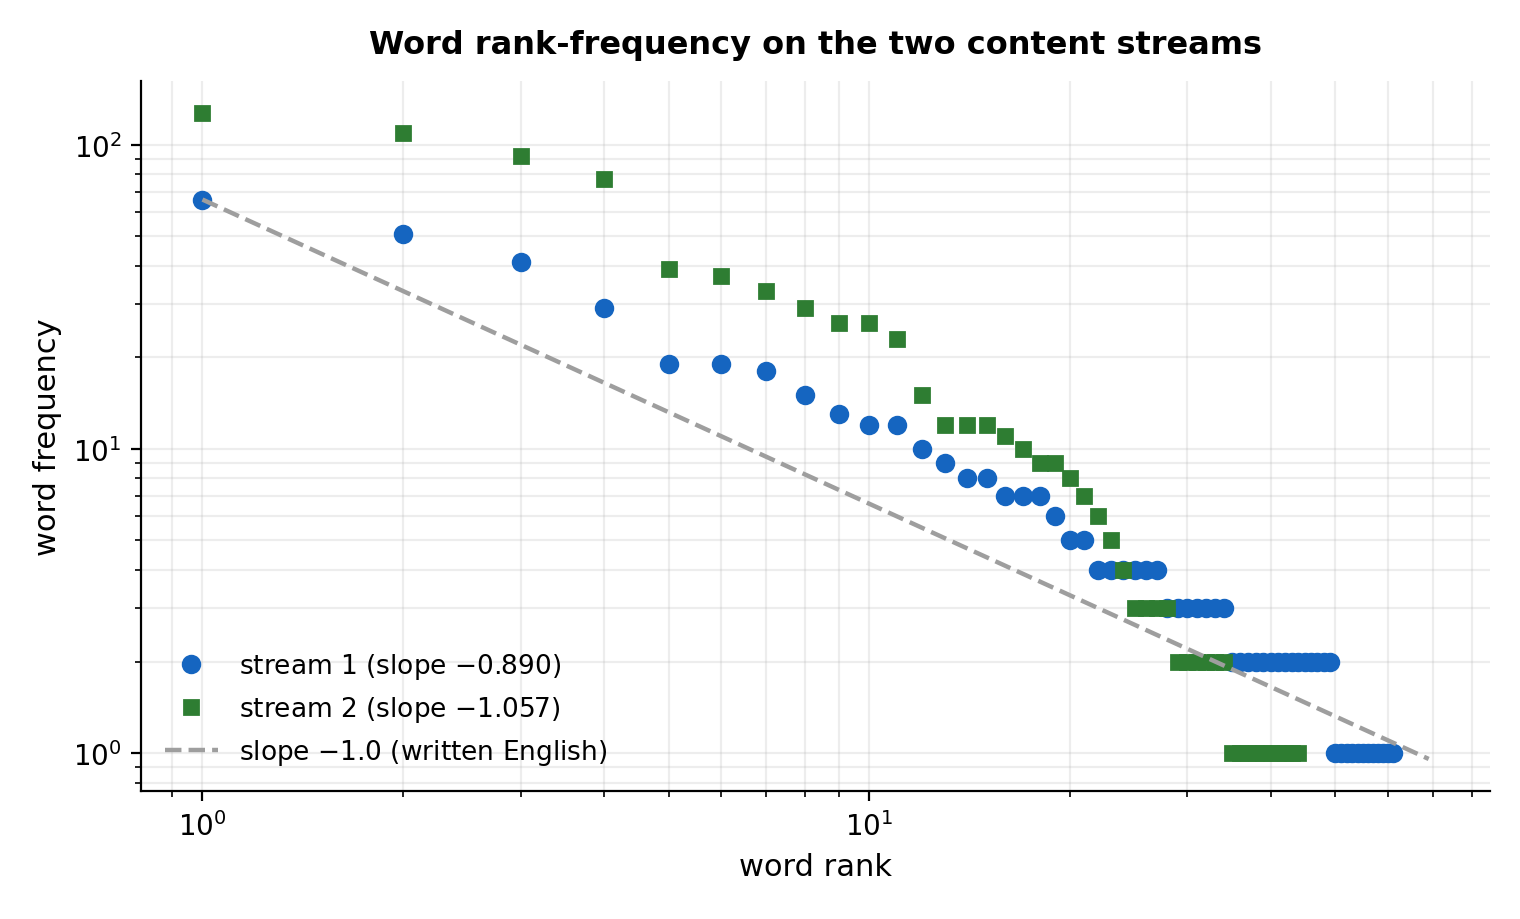
\includegraphics[width=0.8\textwidth]{fig05_zipf_plots.png}
\caption{Zipf rank-frequency distributions for both spectral streams against the ideal
language slope of $-1.0$.}
\label{fig:zipf}
\end{figure}

\subsection{The second axis: depth}
\label{sec:depth}

Section~\ref{sec:direct} established that the standard test has two axes, and the
preceding table reports one of them. Here is the other, on the same object.

Both spectral streams are 4-symbol sequences of length 1863, which is exactly the object
lagged pairwise mutual information is estimable on: the bias floor is 0.0035 bits against
a measured lag-1 value of 0.813 bits. We scan every lag out to 40, past the 32-symbol
frame, because the choice of scan window is a choice and a short one cannot distinguish
absence of structure from absence of looking.

\begin{table}[htbp]
\centering
\caption{Depth on the layer that passes, against the transport layer it was extracted
from. \emph{Depth} is the deepest lag at which prior context still reduces uncertainty at
$z > 3$; \emph{contiguous} is the unbroken run from lag 1. The matched-pipeline English
row is \emph{measured} here, not imported: letters coarsened to a frequency-balanced
four-symbol alphabet, 50 contiguous windows of $N = 1863$, identical estimator and
identical null; the literature rows are Shannon-order references.}
\label{tab:depth}
\small
\begin{tabular}{lrrrr}
\toprule
 & lag-1 MI & lag-1 $z$ & contiguous depth & deepest lag \\
\midrule
spectral stream 1 & \bnum{0.813} bits & \bnum{487} & \bnum{18} & 40 \\
spectral stream 2 & 0.355 bits & 229 & 8 & 35 \\
\midrule
\emph{written English, matched pipeline} & & & \emph{$2.3 \pm 0.8$} & \emph{$8.8 \pm 10.7$} \\
\emph{written English, literature} & & & \emph{$\sim 9$} & \\
\emph{bottlenose dolphin} & & & \emph{$\sim 4$} & \\
\emph{Vela pulsar} & & & \emph{$\sim 0$} & \\
\bottomrule
\end{tabular}
\end{table}

\textbf{Stream 1 reaches an unbroken depth of 18: eight times English measured under
the identical pipeline} ($2.3 \pm 0.8$). A significance-defined span depends on sample
size, alphabet, estimator and null, so the like-for-like comparison is measured rather
than imported; the literature's $\sim$9 for English is a Shannon-order figure, a
different parameterisation, and we do not compare across quantities. Its $z$ falls monotonically from 487 at lag 1 to 2.5 by lag 19. Stream 2
reaches 8, between the matched-English and literature references.

\begin{figure}[htbp]
\centering
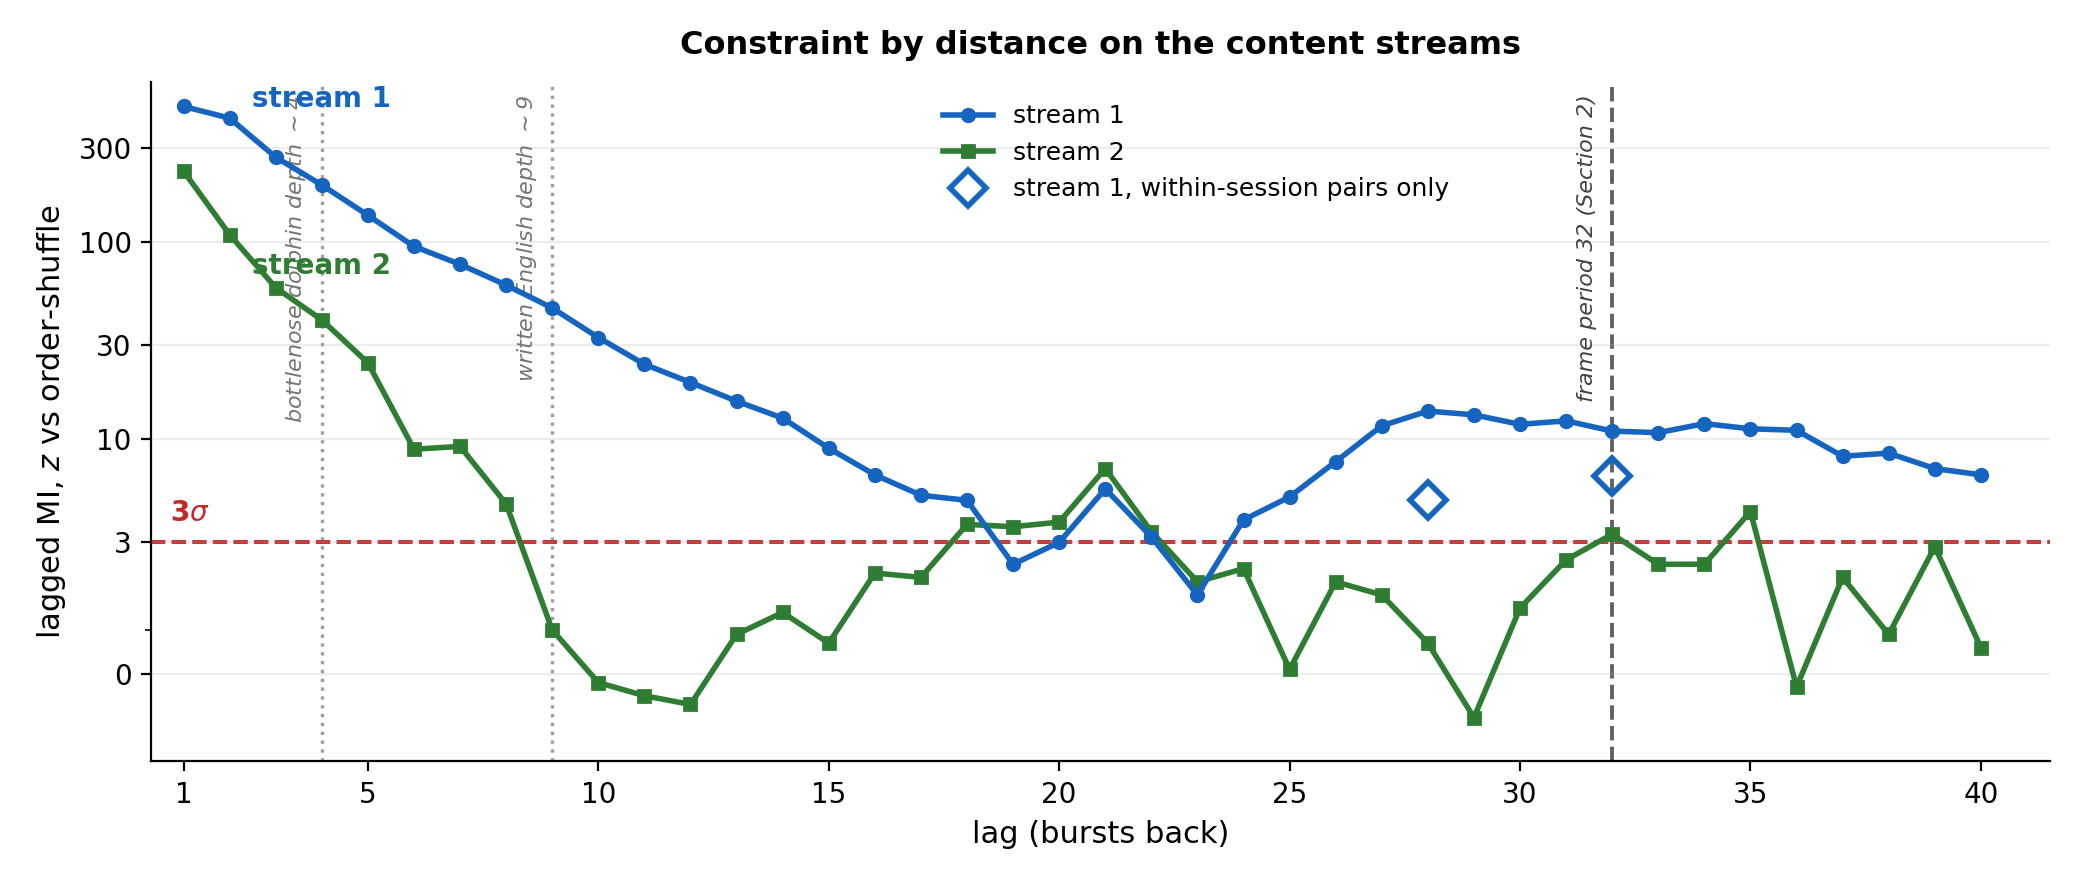
\includegraphics[width=\textwidth]{fig_depth_profile.png}
\caption{The second axis of the language test, in the presentation the
communication-complexity literature uses \cite{mccowan1999,doyle2011}: sequential
constraint by distance on both content streams, $z$ of lagged mutual information
against order-shuffled surrogates (log scale above the linear region; the dashed line
is the $3\sigma$ detection threshold). Stream 1 decays smoothly through the dolphin
and written-English reference depths to an unbroken 18. After touching noise near
lag 19 it returns to a sustained band across lags 24--40, peaking at lag 28 and
holding at the 32-symbol frame period detected independently in
Section~\ref{sec:frame}. Open diamonds: the identical statistic computed on
within-session burst pairs only, against a session-preserving null ($z = +4.9$ at
lag 28, $+6.5$ at lag 32), which separates the band from session-scale drift. Every
value is printed by the analysis script.}
\label{fig:depthprofile}
\end{figure}

\paragraph{A resurgence at the frame period, and the control that identifies it.} The
profile does not simply decay (Fig.~\ref{fig:depthprofile}). After falling to noise
near lag 19, stream 1's mutual
information \textbf{returns}, to a sustained band averaging $z = 9.8$ across lags 24--40
and peaking at $z = 13.9$ at lag 28, with $z = 11.0$ at lag 32. We report this because it
is real and because a summary statistic averaged over lags 5--15, of the kind used in
Table~\ref{tab:direct}, cannot see it.

Two explanations are available and they are separable. The mundane one is drift across
observing sessions: these 1863 bursts span 45 sessions, and slow instrumental or source
evolution would couple distant bursts without any frame. The other is the 32-symbol frame
itself, still visible in the content after demultiplexing.

Restricting to burst pairs \emph{within a single observing session} decides it, against
a null that permutes only within sessions, so session identity and per-session symbol
composition are preserved. At lag 32, within-session mutual information is 0.0689 bits
at $\mathbf{z = +6.5}$ on 626 pairs; at lag 28, 0.0494 bits at $z = +4.9$ on 734 pairs.
\textbf{The long-range structure is not session drift.} It survives inside sessions, at
the frame period, measured on the content layer by a statistic entirely independent of
the sinusoid fit that derived the frame in Section~\ref{sec:frame}.

\subsection{Predictability, measured fairly}

Redundancy $1 - \mathrm{CE}(k)/\mathrm{CE}(0)$ is a ratio, so it compares across
alphabets, but only at matched order, alphabet and estimator. English letters coarsened
to a frequency-balanced four-symbol alphabet and sampled at the matched length, 200
contiguous windows of $N = 1863$, against stream 1:

\begin{table}[htbp]
\centering
\caption{Fraction of the signal predictable from $k$ prior symbols, matched conditions.}
\label{tab:redundancy}
\begin{tabular}{rrrr}
\toprule
order & FRB stream 1 & English & ratio \\
\midrule
1 & \bnum{44.2\%} & $1.6 \pm 0.5$\% & $\mathbf{28\times}$ \\
2 & \bnum{46.5\%} & $4.0 \pm 1.1$\% & $\mathbf{12\times}$ \\
\bottomrule
\end{tabular}
\end{table}

The coarsening itself is not the explanation of English's low score: optimising the
26-to-4 balanced partition \emph{for} English on held-in text, then scoring the
optimised mapping on unseen text, raises English only to $2.5 \pm 0.4$\% at order 1:
the held-out search found no balanced partition approaching the signal. Against Shannon's own measurements for
English \cite{shannon1951} ($h_0 = 4.03$, $h_1 = 3.32$ bits/letter, order-1 redundancy
17.6\%), the stream's 44.2\% is $2.5\times$ English at the same order. Greater predictability is not in itself a mark of
language, and Section~5.4 shows that the redundancy \emph{level} is reproduced by
persistence. What the comparison establishes is that no appeal to insufficient structure
is available against this signal.

\subsection{A recurrent internal vocabulary}
\label{sec:recurrentforms}

The preceding tests establish corpus-level laws and long-range ordering. A separate
question is whether the continuous stream contains reusable internal forms that remain
distinguishable across observing sessions. The test is chronological. Six continuous
phase-path templates---C1, C2, R1, R1+R2, R2 and R3---are fixed from 37 events in the
earlier sessions. At the supplied boundaries of 30 events in later sessions, each event
is assigned to its nearest frozen template. Later labels alter neither the templates nor
the decision rule.

The six templates classify \bnum{21 of 30 later events correctly (70.0\%)}. A
20{,}000-replicate label permutation preserving the width distinction that could make
C1 artificially easy has median accuracy \bnum{26.7\%}; one replicate in 20{,}000
reaches the observed value (exceedance rate $\mathbf{0.00005}$; plus-one Monte-Carlo
$p \approx 10^{-4}$). Early-session accuracy is 70.3\%,
so the inventory retains essentially the same discrimination after the chronological
split. Classification uses normalized continuous phase trajectories, not literal
four-state words.

The boundaries in this test are supplied independently; automatic discovery of every
boundary is a separate segmentation problem. What this experiment establishes is the
identity question: once an event is located, several recurrent internal forms remain
recognisable across time. The stream therefore has both levels required by the
operational grammar definition above: reusable units and long-range higher-order
organization.

The same question has been put to the third source, and the answer has the shape the
rest of this paper's cross-source record leads a reader to expect. FRB~20220912A
independently yields its own recurrent continuous families, widths 5 to 7, with
early-to-later chronological transfer inside that source; literal templates do
\emph{not} transfer between sources, and a template frozen on one source and carried
to the other matches significantly \emph{below} that source's own within-source
control. The architecture replicates while the vocabulary stays source-specific, and
the shared layer has specific content: both sources independently require recurrent,
state-conditioned continuous events that their own background models cannot supply;
both independently recover a primitive-tag-plus-residual-path organization; and both
divide their operations into state-changing and state-preserving roles. The record's
own claim ladder marks this as shared architecture, with every stronger rung, shared
machine invariants, shared composition laws, shared content, explicitly not yet
reached. That combination, common machinery with source-specific expression, is what
distinct installations of one system produce, and it is the opposite of what a shared
instrumental artifact would produce, since both sources were observed with the same
telescope. The cross-source record and its scripts sit
beside the detector cited in the availability section.

\crossbox{The grammar result}{The global tests show that distant parts of the stream
remain related and that combinations carry information unavailable from isolated
symbols. The recurrent-form test identifies stable units: six complex
forms learned earlier are recognized again later at nearly three times the matched
random-label rate. In ordinary terms, the delivered information has a vocabulary, and
the stream those forms live in has long-range combination rules. The two are measured
at different grains, symbol and form; a rule system written over the six forms
themselves is the natural next measurement. Reusable units embedded in consequentially
ordered structure is grammar in the operational sense this paper defines.}

\subsection{Separation is what makes the signal measurable}

\begin{table}[htbp]
\centering
\caption{FRB~20201124A read two ways, one source throughout. The outer and inner layers
of the same signal have opposite statistical signatures.}
\label{tab:progression}
\begin{tabular}{llrr}
\toprule
layer & read & Zipf slope & growth \\
\midrule
outer (transport) & bulk burst parameters & $\mathbf{-0.141}$ & --- \\
inner (content) & spectral stream 1 & $-0.890$ & 0.507 \\
inner (content) & spectral stream 2 & $\mathbf{-1.057}$ & 0.400 \\
\emph{reference} & \emph{written English} & \emph{$-1.00$} & \emph{0.50} \\
\bottomrule
\end{tabular}
\end{table}

\begin{figure}[htbp]
\centering
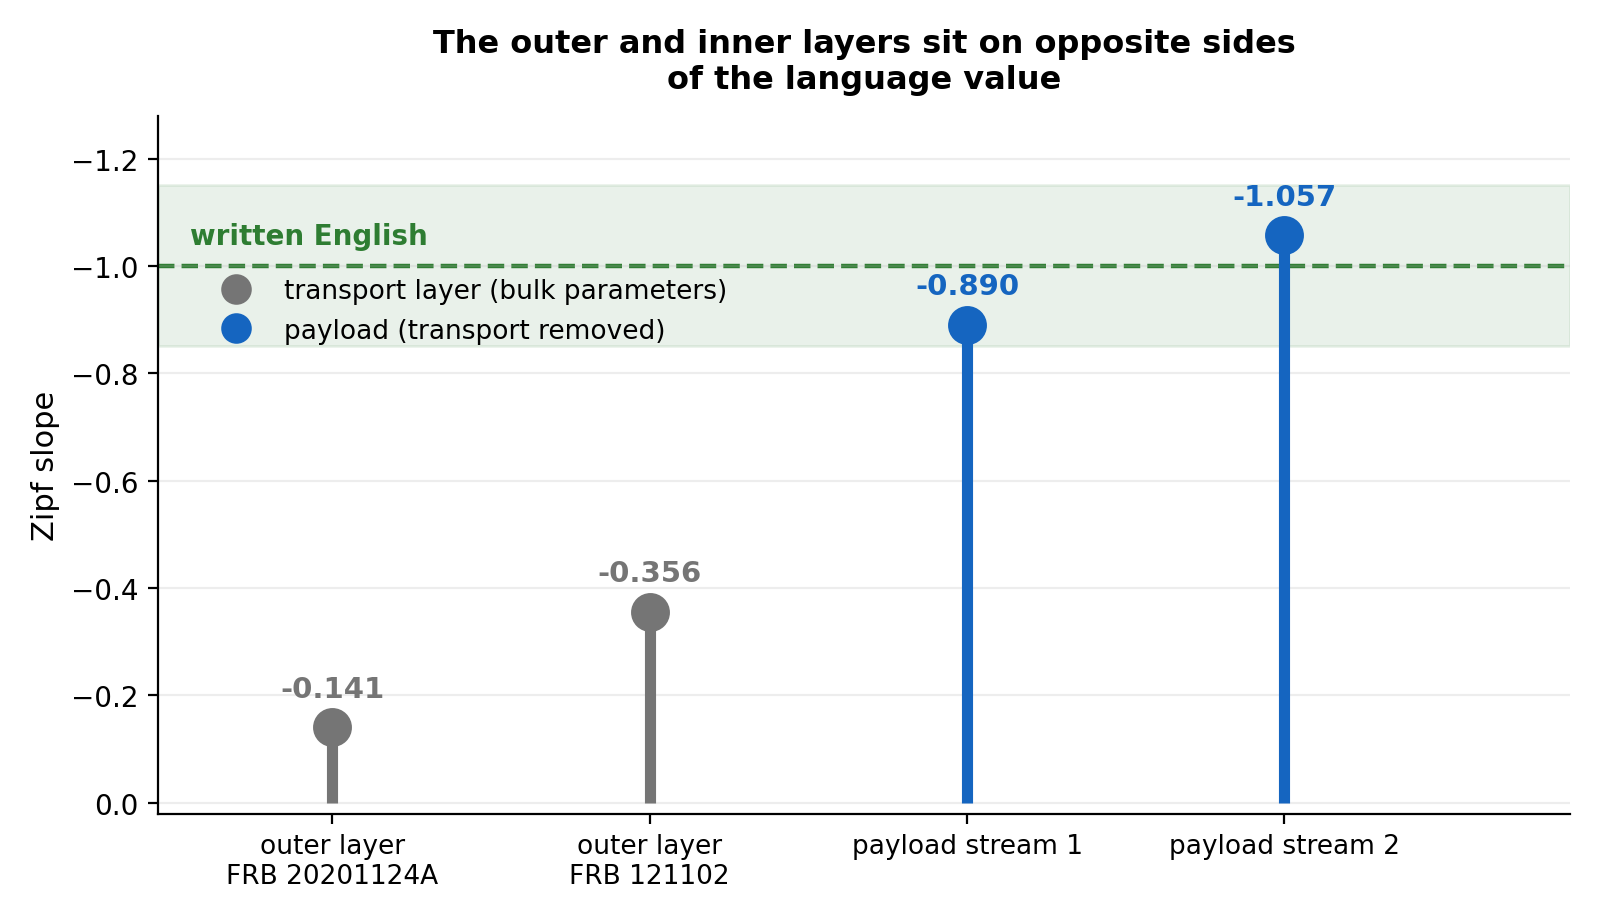
\includegraphics[width=0.74\textwidth]{fig_progression.png}
\caption{The central result. The outer transport layer and the inner content layer sit
on opposite sides of the written-English value; FRB~121102's outer layer, measured
identically, confirms the transport side independently. All four values are printed by
the analysis script.}
\label{fig:progression}
\end{figure}

This is the two-layer architecture of every digital communication system: uniform,
content-agnostic framing wrapped around power-law distributed content. The linguistic
signal was not absent from the raw stream. It was in a different layer of it, and
measuring the two together returns their average.

\section{Controls}
% ============================================================================

The nulls in this section are the ones the comparison literatures use, in their kind
and in their number. The order shuffle is the animal-communication literature's
standard control \cite{mccowan1999,doyle2011}; the goodness-of-fit protocol is the one
the power-law literature prescribes \cite{clauset2009,corral2020}; the
memoryless-marginal control is Sproat's own decisive test \cite{sproat2014}; the
persistence-matched surrogate answers the one remaining mundane reading of this
particular signal. Each is the standard answer to a named, published objection, and we
stack no others: a battery of bespoke falsification attempts distorts as surely as
none, and the point of borrowed methods is borrowed calibration. Throughout, $z$
denotes standardised separation from the surrogate mean, not a Gaussian tail
probability read from hundreds of standard deviations; the empirical exceedance counts
reported alongside are the permutation statement, bounded by the number of surrogates
run.

\subsection{Zipf by maximum likelihood, with goodness of fit}

An ordinary least-squares slope on log-log rank-frequency cannot say whether the data
obey a power law at all \cite{clauset2009}, and rank-frequency is the wrong
representation to fit \cite{corral2020}. Fitting the size distribution by maximum
likelihood with $x_{\min}$ estimated and a parametric bootstrap:

\begin{table}[htbp]
\centering
\caption{Maximum-likelihood power-law fit, implemented as Clauset et al.\ prescribe
\cite{clauset2009}: full $x_{\min}$ scan, semiparametric bootstrap, every synthetic
dataset re-fitted with its own $x_{\min}$ and $\alpha$. Threshold for plausibility is
$p > 0.1$.}
\label{tab:mle}
\begin{tabular}{lrrrrl}
\toprule
 & $\alpha$ & KS $D$ & goodness-of-fit $p$ & tail $n$ & \\
\midrule
spectral stream 1 & \bnum{2.498} & 0.090 & \bnum{0.855} & 11 & not rejected \\
spectral stream 2 & 2.386 & 0.095 & \bnum{0.852} & 11 & not rejected \\
\emph{written English} & \emph{2.00} & & & & \\
\bottomrule
\end{tabular}
\end{table}

The fit does not reject a power law for either stream, and we do not lean on it
further. At this corpus size the fitted tails are small, the exponent is
scan-sensitive (a restricted scan with a 15-point tail floor gives $\alpha = 2.203$
and $1.804$ with $p = 0.900$ and $0.545$), and the lognormal alternative is not
separable (Vuong $p \approx 0.2$): exactly the small-sample behaviour Clauset et al.\
describe. The Zipf evidence in this paper rests on the slope, the order shuffle and
the Markov surrogate, not on this fit; even real English books mostly fail strict
full-domain Zipf protocols \cite{moreno2016}, which calibrates how little a single
fit should be asked to carry.

\subsection{Shuffle the order, keep the bursts}

Every spectrum intact; only \emph{which burst comes when} is shuffled; the entire
pipeline reruns including the PCA, 200 times.

\begin{table}[htbp]
\centering
\caption{Order-shuffle null. Every property of the bursts is held fixed and exactly one
thing varies.}
\label{tab:shuffle}
\small
\begin{tabular}{lccc}
\toprule
 & redundancy & Zipf & growth \\
\midrule
spectral stream 1 & $0.442$ vs $0.002$, $z = \mathbf{512}$
                 & $-0.890$ vs $-2.139$, $z = \mathbf{12.5}$
                 & $0.507$ vs $0.203$, $z = \mathbf{7.9}$ \\
spectral stream 2 & $0.187$ vs $0.002$, $z = \mathbf{234}$
                 & $-1.057$ vs $-2.161$, $z = \mathbf{12.1}$
                 & $0.400$ vs $0.199$, $z = \mathbf{4.5}$ \\
\bottomrule
\end{tabular}
\end{table}

\textbf{The shuffled signal is not merely flattened, it is specifically wrong.} A Zipf
slope near $-2.15$ lies far outside the range reported for human language corpora, and a
vocabulary growth near $0.20$ is a closed, fixed word set. Shuffling does not erase the
pattern; it replaces it with the signature of a degenerate code. Every language-grade
value exists only in the original temporal order.

\subsection{The memoryless-marginal control}
\label{sec:memoryless}

The strongest published objection to entropy-based inference is that a memoryless
sequence drawn from a skewed symbol distribution can land inside the language range on
\emph{absolute} conditional entropy \cite{sproat2014}: a low $H(x_t \mid x_{t-1})$ may
reflect nothing but an uneven marginal.

The objection is real and it is also self-limiting. For an i.i.d.\ sequence
$H(x_t \mid x_{t-1}) = H(x_t)$ exactly, so $I(x_t; x_{t-1}) = 0$ and \textbf{every
conditional-entropy reduction is zero by construction}. The control that defeats an
absolute-entropy claim cannot touch a reduction claim. Built from our own marginal:

\begin{table}[htbp]
\centering
\caption{Real sequence against an i.i.d.\ control with the identical symbol
distribution. Matched to three decimals at order 0; separated by 0.8 bits at every order
above.}
\label{tab:memoryless}
\begin{tabular}{rrrrrr}
\toprule
$k$ & real $h_k$ & i.i.d.\ control & \bnum{gap} & $z$ & controls beating real \\
\midrule
0 & 1.839 & 1.839 & 0.000 & 0.0 & 98/200 \\
1 & 1.027 & 1.834 & \bnum{0.807} & \bnum{48.4} & \bnum{0/200} \\
2 & 0.985 & 1.819 & \bnum{0.834} & \bnum{54.2} & \bnum{0/200} \\
3 & 0.946 & 1.759 & \bnum{0.813} & \bnum{50.4} & \bnum{0/200} \\
\bottomrule
\end{tabular}
\end{table}

Under a bias-immune held-out estimator, where running short of data makes a model score
\emph{worse} rather than artificially better, the separation persists undiminished:
$0.786 \rightarrow 0.799 \rightarrow 0.843 \rightarrow 0.861 \rightarrow 0.807$ bits at
orders 1 through 5, rising through order 4.

\subsection{A null that reproduces the persistence}
\label{sec:markov}

The controls above establish that temporal order matters. They do not, by themselves,
separate protocol-grade structure from ordinary first-order persistence, and this
matters here more than usual: the stream holds its state 75.7\% of the time and words
are defined as maximal runs, so run-length statistics follow directly from persistence.

The decisive null is therefore a surrogate that reproduces persistence exactly. We fit
the full $4 \times 4$ transition matrix to each real stream and generate order-1 Markov
realisations from it. These match the symbol marginal, the transition matrix, and hence
the implied run-length law by construction. The full pipeline is rerun on each of 300
realisations.

\begin{table}[htbp]
\centering
\caption{Both spectral streams against an order-1 Markov surrogate matched on
persistence and its implied run-length statistics. The redundancy \emph{levels} are
fixed by construction; the vocabulary structure and the predictability gain, in bits,
are not.}
\label{tab:markov}
\small
\begin{tabular}{llrrrr}
\toprule
 & measure & real & Markov-1 surrogate & $z$ & exceedances \\
\midrule
 & \multicolumn{5}{l}{\textbf{stream 1}} \\
 & \bnum{predictability gain $G_1$} & \bnum{0.0418} & $0.0128 \pm 0.0031$ & $\mathbf{+9.4}$ & \bnum{0/300} \\
 & \bnum{Zipf slope} & $\mathbf{-0.890}$ & $-0.660 \pm 0.055$ & $\mathbf{-4.2}$ & \bnum{0/300} \\
 & \bnum{vocabulary growth} & \bnum{0.507} & $0.412 \pm 0.041$ & $\mathbf{+2.3}$ & \bnum{5/300} \\
 & \bnum{word types} & \bnum{61} & $55.6 \pm 2.6$ & $\mathbf{+2.0}$ & \bnum{8/300} \\
 & \emph{brevity} & \emph{$-0.800$} & \emph{$-0.858 \pm 0.028$} & \emph{$+2.1$} & \emph{293/300} \\
 & \emph{redundancy, order 1} & \emph{0.442} & \emph{$0.442 \pm 0.016$} & \emph{$-0.0$} & \emph{145/300} \\
\midrule
 & \multicolumn{5}{l}{\textbf{stream 2}} \\
 & \bnum{predictability gain $G_1$} & \bnum{0.0428} & $0.0146 \pm 0.0034$ & $\mathbf{+8.4}$ & \bnum{0/300} \\
 & Zipf slope & $-1.057$ & $-0.973 \pm 0.050$ & $-1.7$ & 10/300 \\
 & \bnum{vocabulary growth} & \bnum{0.400} & $0.294 \pm 0.035$ & $\mathbf{+3.1}$ & \bnum{1/300} \\
 & \bnum{word types} & \bnum{44} & $38.2 \pm 2.1$ & $\mathbf{+2.8}$ & \bnum{2/300} \\
 & \emph{brevity} & \emph{$-0.921$} & \emph{$-0.909 \pm 0.021$} & \emph{$-0.6$} & \emph{93/300} \\
 & \emph{redundancy, order 1} & \emph{0.187} & \emph{$0.189 \pm 0.013$} & \emph{$-0.2$} & \emph{167/300} \\
\bottomrule
\end{tabular}
\end{table}

Read the table in two parts, because the first part is easy to misread.

\textbf{The italicised rows are a validity check on the surrogate, not a null result.} A
reader will see real 0.442 against surrogate 0.442 at $z = 0.0$ and conclude that the
surrogate has defeated the redundancy claim. It has done the opposite: it has demonstrated
that it works. Order-1 redundancy $1 - h_1/h_0$ is a deterministic function of the symbol
marginal and the transition matrix, and both were measured on the real stream and then
used to build the surrogate. Matching is arithmetic, not evidence, and a surrogate that
failed to match here would be misconfigured. Brevity is in the same category for the same
reason: it is a statistic of the run-length law, which the surrogate fixes in
expectation, so it cannot discriminate here and we do not ask it to. The correct
reading of these rows is ``the control is correctly calibrated'', which is what licenses
the rest of the table.

\textbf{What the surrogate cannot reproduce is the higher-order information.} The
predictability gain of the second-order context,
$G_1 = h_1 - h_2 = I(x_t; x_{t-2} \mid x_{t-1})$ \cite{degregorio2026}, is
the quantity that directly answers ``is this just persistence?'', because it measures
what a more distant symbol adds \emph{given} the nearer one. It exceeds the surrogate at
$\mathbf{z = +9.4}$ on stream 1 and $\mathbf{z = +8.4}$ on stream 2, roughly three times
the surrogate's value in both cases. \textbf{The answer is no, and it is not close.}

The vocabulary structure is likewise not reproduced: stream 1's Zipf slope in
\bnum{0 of 300} attempts, stream 2's vocabulary growth in \bnum{1 of 300}. Stream 2's
Zipf slope is the one measure the surrogate approaches ($z = -1.7$, 10/300), and we
report that rather than omit it.

This is the strongest control we can construct against the persistence explanation, and
the signal clears it by an order of magnitude on the measure built for the purpose.

Order shuffles and Markov surrogates are statistical nulls. A separate question is
whether a physically correlated emitter could produce the observed sequential
structure, and the source analysis \cite{meucci2026} addresses it directly with two
tests we summarise rather than recompute here.

First, a multivariate Ornstein--Uhlenbeck process, the standard model for a source
relaxing toward a mean with exponentially decaying memory, calibrated to the
\emph{exact} measured cross-lag correlation matrix of the real data. It reproduces a
large part of the observed structure, mutual information $0.093$ bits against the real
$0.125$, and the real data still exceeds it ($z = 2.02$, $p = 0.03$). This is a
deliberately generous null and the margin over it is correspondingly modest.

Second, and more decisive, the residual test. Burst energy, width and bandwidth are
physically coupled. Regressing width and bandwidth on energy and testing the residuals
isolates variation that the dominant physical variable cannot explain. Those residuals
retain sequential structure at $\mathrm{MI} = 0.033$ bits against a shuffled baseline of
$0.004$: $z = 14.44$ on the FAST sample of FRB~121102 ($n = 1652$) \cite{li2021}. The
same residual test replicates at $z = 2.95$ on the independent Arecibo sample of the
same source ($n = 144$) \cite{aggarwal2021} and at $z = 3.16$ on FAST FRB~20201124A
($n = 1863$) \cite{wang2023}: jointly $p = 4.8\times10^{-7}$, \textbf{5.0$\sigma$
across three datasets, two telescopes and two sources} \cite{meucci2026}.

These answer a different question from the spectral $z$-scores in Section~2.1. The
large $z$ values establish that structure exists in the channels; the residual test
establishes that it is not reducible to a single physical state variable driving all
burst parameters together.

\paragraph{One claim we withdraw, by the same standard.} The source analysis, and an
earlier version of this paper, additionally reported near-perfect symbol
equiprobability in the outer layer, 25\% per symbol at a coefficient of variation
below 0.003, as evidence of a channel optimised for capacity. \textbf{We drop it.}
Those symbols are defined as quantiles of the burst parameter distribution, so equal
occupancy is guaranteed by the binning and measures nothing about the signal. It is
the same defect this section identifies in the Markov redundancy match
(Section~\ref{sec:markov}) and we hold ourselves to it. The flat Zipf slope of the
outer layer, $-0.141$, is the sound form of the same observation: it is computed on
the joint nine-state symbol distribution, whose occupancies are not fixed by the
marginal tercile construction.

\subsection{The measurement is far inside its limits}

Maximum reliable order for block conditional entropy is
$r_{\max} = \lfloor \ln N / \ln K \rfloor$ \cite{degregorio2026}. At $N = 1863$, $K = 4$
this is 5, and every claim above is at order $\leq 3$. The plug-in mutual-information
bias floor, $(K-1)^2/2N$ \cite{paninski2003}, is \bnum{0.003 bits} against a measured
lag-1 value of \bnum{0.813 bits}: a \bnum{270-fold margin}. These numbers are not
squeezed out of a starved estimator.

% ============================================================================
\section{Cross-source replication}
% ============================================================================

Two distinct things are often conflated under ``replication'', and they carry very
different weight. We separate them.

\paragraph{Prospective prediction.} The analysis framework was developed on two FRB
sources. A third, FRB~20220912A, became available afterwards. Seven quantitative
predictions were stated and then tested against it \emph{before} any parameter
adjustment. \textbf{Every one that could be tested on that source was confirmed.} The
seventh, bulk vocabulary growth, has no object at FRB~20220912A: the archive provides 894
dynamic spectra and no bulk parameter table, so the quantity predicted does not exist
there. The spectral-layer value is given in its row for completeness and is a
retrospective, not prospective, comparison.

\begin{table}[htbp]
\centering
\caption{Predictions stated before FRB~20220912A was analysed, and their outcomes.
This is the strongest methodological feature of the work: the model could not have been
tuned to data it had not seen.}
\label{tab:predictions}
\small
\begin{tabular}{llll}
\toprule
prediction & predicted & observed & \\
\midrule
Brevity $\rho$ & $-0.94 \pm 0.05$ & $-0.883$ & confirmed (within $2\sigma$) \\
Zipf slope & $-0.8$ to $-1.1$ & $-1.057$ & confirmed \\
Same 4-sector phase structure & yes & yes & confirmed \\
All spectral channels above null & yes & $z = 196$--$338$ & confirmed \\
Sinusoidal 32-offset fit & $r > 0.5$ & $r = 0.595$, $p = 0.0003$ & confirmed \\
Anti-synchronised transitions & yes & yes & confirmed \\
Vocabulary growth $\beta$ & $0.373 \pm 0.02$ & 0.523 (spectral layer) & no object at source \\
\bottomrule
\end{tabular}
\end{table}

The rows carry unequal weight, and we rank them before a reader does. The Zipf
bracket, the spectral-channel significances, the 32-offset profile and the
anti-synchronised transitions are quantitative predictions that could readily have
failed. The four-sector structure is partly fixed by the quadrant construction, and
brevity is substantially induced by run-length encoding (Section~\ref{sec:markov}).
Six of six is the count; four hard quantitative hits are the evidence.

\paragraph{Recomputed here, on the archive as it stands.} The prediction table is the
historical record, and later data cannot change it. Separately, our script re-runs the
source analysis's pipeline for this source on the 949 spectra now public; the original
run used the 894 then available \cite{zhang2023}. The architecture replicates: a
dominant carrier (76\% of variance) wrapping components that all carry sequential
structure at $z = 201$--$335$ (original run: 196--338), and the 32-offset wave profile
persists at the same period ($r = 0.496$, $p = 0.004$). The linguistic values on the
grown archive: Zipf slope $-1.143$, vocabulary growth $0.540$, brevity $-0.850$. We
print these as they fall: on today's larger archive the wave-fit point estimate sits
below the pre-registered $r > 0.5$ threshold while remaining significant at the same
period, and the Zipf slope steepens slightly past the predicted bracket. The carrier,
the channel structure and the frame profile are the replicated architecture.

\paragraph{Retrospective cross-source agreement.} Separately, ten protocol and
statistical features were compared across all three sources after the fact:
\textbf{25 of 25 testable cells confirmed, none failed}; five cells are not testable
from the available data (Fig.~\ref{fig:xsource}). This is weaker evidence than the
prospective table, because the features were not committed to in advance, and we label
it as such.

Prediction confirmed on data not used to build the model is worth more than any single
significance value in this paper.

\begin{figure}[htbp]
\centering
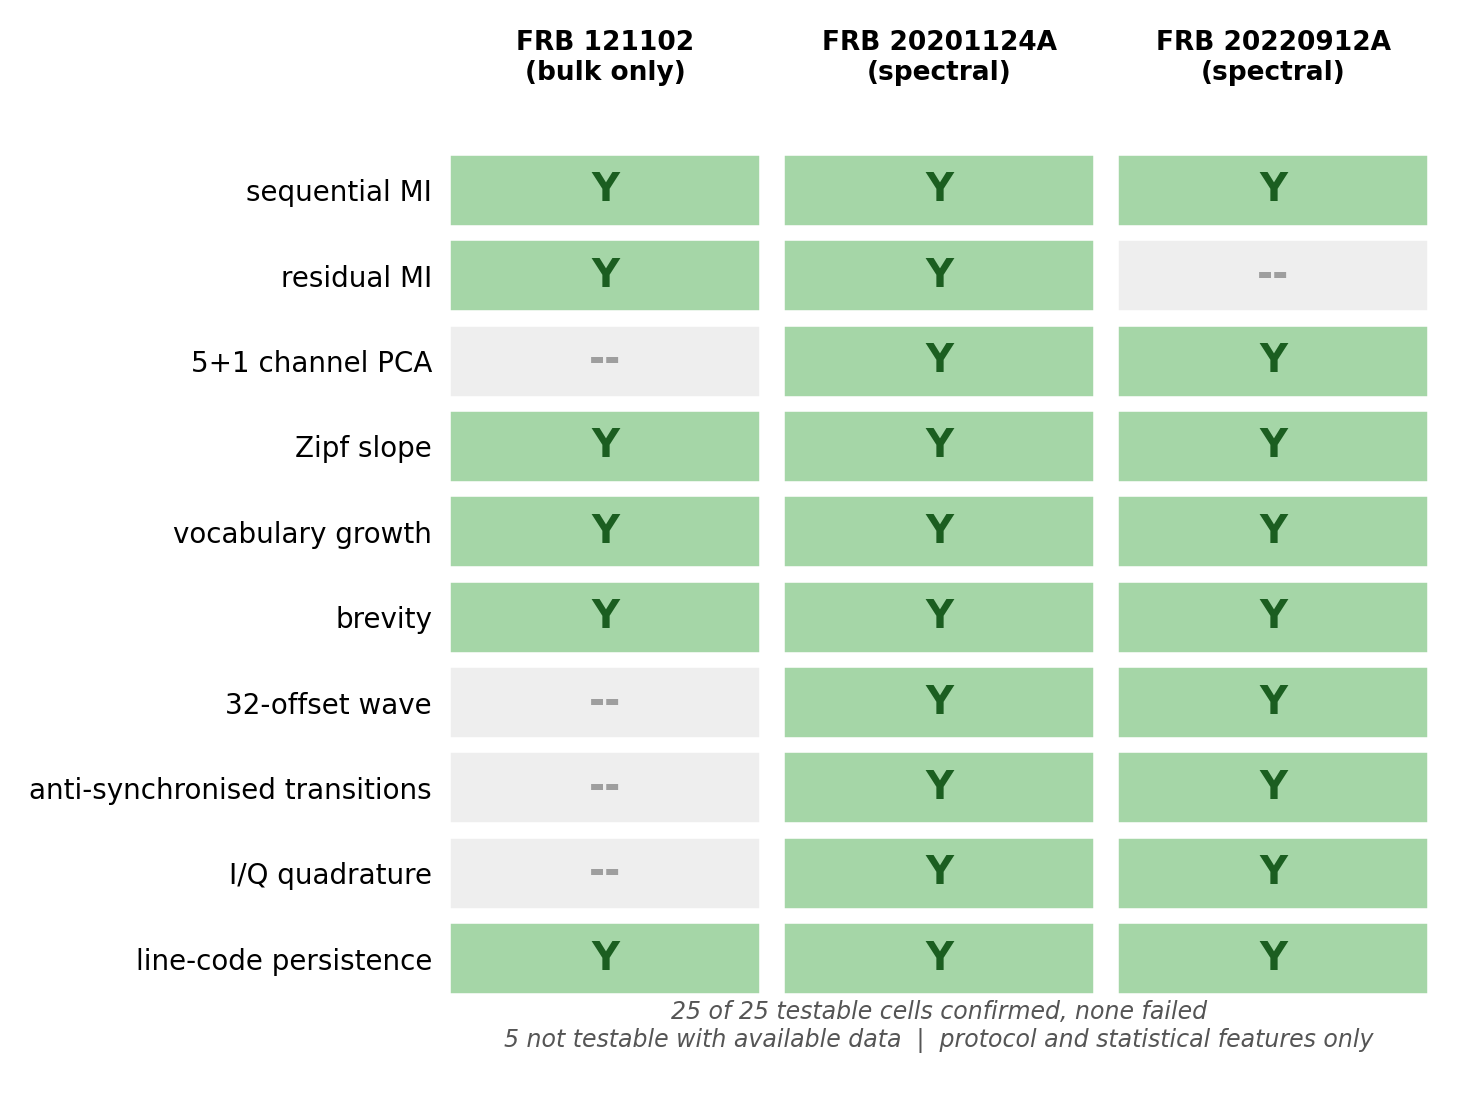
\includegraphics[width=0.80\textwidth]{fig_crosssource.png}
\caption{Retrospective feature confirmation across three independent FRB sources,
restricted to protocol and statistical features; content-interpretation rows from the
source analysis \cite{meucci2026} are excluded as outside this paper's scope. Green
confirmed, grey not testable with the available data for that source. No cell failed.
Compare Table~\ref{tab:predictions}, which is prospective and carries more weight.}
\label{fig:xsource}
\end{figure}

\subsection{The same source through two telescopes: a fingerprint square}
\label{sec:square}

Every payload measurement so far, on all three sources, comes through one instrument
chain: FAST. The remaining objection class is instrumental, that the payload
statistics are a signature of the telescope rather than of the sources. This is testable with public
data, and we tested it with the match criteria fixed before anything was computed.
FRB~121102 is the one source in this paper's set with published burst spectra from a
second major telescope: 404 burst-centred, bandpass-normalised Arecibo arrays from the
2016 burst storm \cite{hewitt2022}, three years before the FAST campaign
\cite{li2021}. That yields a two-by-two design: the same source through two
telescopes, and different sources through the same telescope.

All four datasets, FRB~121102 through Arecibo, FRB~121102 through FAST,
FRB~20201124A and FRB~20220912A through FAST, were reduced to the identical
representation: per-burst spectra on a common 12.5-MHz grid over 1150--1500~MHz, the
band the two telescopes share, then the identical pipeline used everywhere in this
paper (PCA, carrier discarded, the two quadrant streams), then nine stream statistics
per 352-burst window, each invariant under relabeling of the quadrants so that no
dataset's arbitrary PCA orientation can matter. The distance between two datasets is
the median feature difference in units of the within-dataset window scatter.

\begin{table}[htbp]
\centering
\caption{Fingerprint distances between the four datasets: median difference over nine
relabeling-invariant payload-stream statistics, in units of within-dataset window
scatter. The same source through two different telescopes is three to four times
closer than FRB~121102 against either different source through its own telescope
(3.78, 5.47); under the uniform
burst-window extraction of the FAST~121102 cell the same-source distance falls to
\bnum{0.70}, below window scatter, against 4.94 and 6.63. The remaining FAST pair
separates at 1.65: every pair of different sources is resolved, and the closest pair
in the matrix is the same source through two telescopes. All values printed by
\texttt{fingerprint\_square.py}.}
\label{tab:square}
\small
\begin{tabular}{lrrrr}
\toprule
 & 121102/AO & 121102/FAST & 20201124A/FAST & 20220912A/FAST \\
\midrule
121102 / Arecibo    & ---  & \textbf{1.27} & 5.64 & 7.33 \\
121102 / FAST       & \textbf{1.27} & ---  & 3.78 & 5.47 \\
20201124A / FAST    & 5.64 & 3.78 & ---  & 1.65 \\
20220912A / FAST    & 7.33 & 5.47 & 1.65 & ---  \\
\bottomrule
\end{tabular}
\end{table}

Table~\ref{tab:square} is the result. The same source through two different
telescopes: distance 1.27, and \textbf{0.70, below the window scatter itself}, under a
uniform burst-window extraction of the FAST cell. FRB~121102 against different
sources through its own telescope: 3.78 and 5.47 (4.94 and 6.63 under the same
uniform extraction). The third same-telescope pair, FRB~20201124A against
FRB~20220912A, separates at 1.65; every pair of genuinely different sources is
resolved, and the closest pair in the whole matrix is the same source through two
different telescopes. The
control also inverts correctly: if the burst signal is deliberately erased from the
FAST~121102 dataset, by averaging whole files so that a millisecond burst is diluted
over seconds of receiver noise, the dataset stops matching Arecibo~121102 and drifts
toward the other FAST datasets. The telescope's own signature appears exactly and
only when the source's signal is removed.

The payload statistics travel with the source, across telescopes and across a
three-year epoch gap, while genuinely differing between sources observed through the
same instrument; they are modulation-side quantities, not receiver-side ones. An
instrumental account of the payload structure would now need FAST to imprint a
different fingerprint on each source it observes while Arecibo independently imprints
the right one on the one source they share. The caveats are recorded in the companion
script's committed output: the two 121102 datasets supply one 352-burst window each,
so the scatter scale is taken from the larger datasets, and the channel-order
convention is verified against the PSRFITS frequency table for FRB~20201124A and
assumed for the other FAST products.

% ============================================================================
\section{Discussion}
% ============================================================================

\subsection{What the comparison-class literature actually shows}

Sproat \cite{sproat2014} compared written language against weather-forecast icon
sequences, emoticons, mathematical notation, heraldry, totem poles and Mesopotamian
deity symbols. He was asking whether statistics distinguish \emph{writing}, symbols
encoding units of a spoken language, from other symbol systems, and he explicitly
contrasts writing with systems such as traffic signs, music and mathematics that convey
information independently of any language.

His comparison class is therefore \textbf{not a set of noncommunicative controls; it is
mostly a set of combinatorial meaning-bearing systems}. Emoticons are the clean case: no
individual punctuation mark carries the expression the combination produces. Mathematics
is unambiguous, since the relations among symbols \emph{are} the proposition. So the
result is not that these statistics are empty. It is that they identify a \emph{class}
of which written language is one member. Membership is a substantive finding.

Four points bound what the study established. Its classifier contained \textbf{no Zipf
feature}, so Zipf's known weakness was never bundled with conditional entropy. Its
conditional-entropy curve holds conditioning at one symbol and expands the
\emph{vocabulary}, making it a vocabulary-growth curve rather than $h_1, h_2, h_3$; and
its block entropies test \emph{levels} $B(k)$, whereas depth lives in the
\emph{increments} $h_k = B(k{+}1) - B(k)$, which two corpora can differ in while
agreeing on the sum. Its inscriptions averaged 1.4 to 13.6 symbols against 6-symbol
blocks. \textbf{Depth was never measured.} And its conclusion was not that
classification is impossible: a modified cut-off and a new repetition measure classified
the categories successfully. Section~\ref{sec:memoryless} runs its decisive control
directly and passes at $z = 48$--$54$ with zero exceedances.

\textbf{This framing is the published standard.} \emph{Science} carries ``Whale song
shows language-like statistical structure'' \cite{arnon2025} and \emph{Nature
Communications} carries ``Contextual and combinatorial structure in sperm whale
vocalisations'' \cite{sharma2024}. Both are post-Sproat, both in top-tier venues, and
both claim exactly what we claim: combinatorial statistical structure, not natural
language. We hold ourselves to that standard and meet it with larger margins.

\subsection{The language finding has two scales}

The global and internal results are not separate curiosities. Zipf and vocabulary
growth show how forms are distributed across the corpus. Dependency depth and
conditional information show that order carries information across many positions.
The six recurrent continuous forms identify stable units inside that ordered stream.
Together they supply the two observable levels ordinarily meant by grammar: a reusable
inventory and nonlocal rules of combination.

This is stronger than obtaining a language-like rank-frequency slope from an arbitrary
sequence. The units are learned in one chronological block and recognised in another;
the ordering exceeds a surrogate built to reproduce the signal's own persistence and
run-length statistics. The recurrent-form result is the bridge between the corpus-level
laws reported here and a fuller analysis of internal organization, which is reserved
for subsequent work.

\subsection{The direction of the excess}
\label{sec:excess}

Where the payload deviates from written English, it deviates consistently in one
direction: more redundancy (44.2\% against matched English's 1.6\%), a longer
dependency span (18 against 2.3), brevity holding more tightly ($-0.921$ against
$-0.70$). A natural question is whether the direction itself says something about the
\emph{kind} of content, since noise does not overshoot language, but dense, formal,
structured text might. We measured it. Under the identical pipeline, mathematical
prose (Laplace's \emph{Essay on Probabilities}) sits at $1.9 \pm 0.5$\% order-1
redundancy with depth $2.9 \pm 1.4$; structured problem-and-solution text (Dudeney's
\emph{Amusements in Mathematics}) at $2.5 \pm 0.7$\% with depth $2.6 \pm 0.8$.
\textbf{Order-1 redundancy climbs monotonically as English text becomes more formal,
dependency span stays confined near 2--3 throughout, and neither comes anywhere near
the payload.} The gradient runs narrative prose $\rightarrow$
mathematical prose $\rightarrow$ structured mathematics $\rightarrow$ this signal,
with the signal roughly an order of magnitude beyond the structured end. The direction
is consistent with content more formal than any natural-language register; the
magnitude says no English text approaches it. We record this as an observation about
the statistics, not a reading of content: what kind of source sits that far along the
axis that formal text starts down belongs to the experiments of
Section~\ref{sec:further}.

\subsection{A note on non-separable objections}

Three of the most natural objections to this analysis share a structure worth naming,
because each is persuasive on first reading and none of them bites.

\begin{enumerate}[leftmargin=1.6em,itemsep=3pt]
\item \emph{The low entropy at offsets 8--16 is caused by the skewed symbol marginal
there, not by a header.} But a symbol marginal that varies with offset is what a frame
is. The objection relocates the claim from one statistic to another and leaves it
intact (Section~\ref{sec:fields}). The two quantities involved, mean wave-state amplitude
and per-offset entropy, are moreover both summary statistics of the \emph{same}
per-offset symbol distribution, so their high correlation is close to an identity rather
than a confound.
\item \emph{The Markov surrogate reproduces the redundancy, so the redundancy is just
persistence.} But the surrogate was built from the measured transition matrix, and
order-1 redundancy is a deterministic function of it. The match is arithmetic
(Section~\ref{sec:markov}).
\item \emph{The entropy segmentation disagrees with the mutual-information boundaries.}
But coupling seams and low-variability fields are different features and sit at
different offsets in any framed format (Section~\ref{sec:frame}).
\end{enumerate}

The common form is an alternative explanation that is not \emph{separable} from the
claim it is meant to replace. A genuine alternative must be capable of being true while
the claim is false. If asserting it requires asserting the claim, if it appeals to a
quantity that was fixed by construction, or if it requires two statistics measuring
different objects to coincide, it has not competed with the claim at all. Stated
carefully, each of the three concedes the thing it was raised to deny.

We state this not to deflect scrutiny but to direct it. The separable objections are
the ones we have tried hardest to answer, and they are the ones in Section~5: does
temporal order matter, is the vocabulary distribution reproducible from persistence
alone, is an absolute entropy value reproducible from a skewed marginal, and can a
calibrated physical process account for the sequential structure. Those tests can all
come out the other way, and two of them nearly do: stream~2's Zipf slope is approached by
the Markov surrogate ($z = -1.7$, 10 of 300), and the Ornstein--Uhlenbeck null clears only
$z = 2.02$. We report both margins as they fell.

\subsection{On ``but is it \emph{really} language''}

We refuse this question, and we refuse it on principle rather than for want of an answer.

Whether a system that transmits information through rule-governed symbol combinations
also earns the word \emph{language} is a question about the boundaries of an English
term. It is settled by definition, not by measurement, and \textbf{no observation of the
signal can bear on it.} That is not a hard question. It is a question of a kind that
measurement cannot address at all.

We therefore name what is happening when it is demanded as a precondition. \textbf{A
criterion that no possible observation can satisfy, required before measurements are
taken seriously, is not a high standard. It is a bias toward the null wearing the costume
of rigour.} It cannot be met by better data, more surrogates, or a further control,
because nothing in the data is what it is about. Applied consistently it would also
exclude the whale-song results in \emph{Science} and \emph{Nature Communications} that
supply the register for this paper \cite{arnon2025,sharma2024}, and it is not applied to
them. We decline to accept it as a legitimate mode of academic examination of this
subject, and we say so plainly rather than negotiating with it.

The measurable questions are these, and they are ordered:
\begin{enumerate}[leftmargin=1.6em,itemsep=1pt]
\item Is the sequence nonrandom?
\item \textbf{Do combinations carry information not available from the symbols
individually?}
\item Is it a conventional meaning-bearing communication system?
\item Does it encode a natural human language?
\end{enumerate}

Within this paper, \emph{language} is accordingly used the way the toolkit uses it: as
the name of the measured class that questions 1 and 2 pick out, systems whose symbol
combinations carry information their symbols alone do not. Questions 3 and 4 name
different properties. The measurements do not claim them; this edition's
interpretation layer states our assessment of question 3 openly, once, in
Appendix~\ref{app:crossdisciplinary}, labeled as interpretation rather than
measurement. Question 4 is not entered.

\textbf{This paper answers 1 and 2 affirmatively, with margins running from} $z = 8.4$,
against a surrogate built to reproduce the signal's own persistence, \textbf{to}
$z = 512$ against an order shuffle. Question~2 is the substantive one. A system whose combinations carry
information beyond its symbols is doing what mathematics, DNA, music, cetacean song and
written language all do, and there is no well-attested natural system with deep
combinatorial symbolic dependency that is not information-bearing.

Questions 3 and 4 require different evidence, and we say what would supply it:
conditioning one source's output on another's preceding sequence, directional transfer
entropy between them, cross-source replication of the same field layout, and systematic
covariance between symbol combinations and an independently measurable variable. Those
are experiments, and they are the next ones.

\subsection{The ledger against the source analysis}

This paper is a reanalysis, and the reader should not have to reconstruct what
happened to the source analysis's claims \cite{meucci2026}; we state the ledger.
\textbf{Reproduced and retained:} the two-layer architecture; the 32-symbol frame,
taken from the source as pre-specified and here falsified against its sub-periods and
recovered on the native phase; the carrier and its five sub-channels; the payload
streams' two-axis language pass; and the prediction record on FRB~20220912A, kept as
a historical table that later data does not rewrite. \textbf{Strengthened here:} the
channel significances and power-law tables were recomputed from the archives as they
stand today, and both moved \emph{up}; the literature English reference was replaced
by matched-pipeline measurement, which raised the redundancy contrast to
$28\times$; the within-session control was tightened to a session-stratified null and
survived; and the transport/content division gained two controls the source did not
have, the cross-telescope fingerprint square and the 11{,}553-burst bulk null.
\textbf{Withdrawn or not adopted, by our own standard:} the source's
equiprobable-symbol evidence (fixed by the binning, withdrawn in
Section~5); its within-frame field layout (our omnibus test is negative and is
reported as such); and its description of the carrier as featureless (recomputation
finds structure there; for multiplexing the components need to be separable, not the
carrier empty, so this discrepancy is reported and costs nothing).
\textbf{Bracketed, not adjudicated:} the source analysis's content-level reading, the
wave-value arithmetic and the mathematical-primer interpretation built on it, is
question-3-and-4 territory: it is relied on nowhere in this paper, and nothing
measured here tests it or bears on it. It is out of scope by design, not withdrawn
and not endorsed; a separate program of work addresses it. We permit ourselves one
anticipatory remark: the independent continuation of the recurrent-form program of
Section~\ref{sec:recurrentforms}, working from the continuous phase paths rather than
the source analysis's quantized values, appears to be converging on the kind of
object that reading presupposed, a small library of reusable operations whose ordered
compositions construct their outcomes; a follow-up paper will put that account under
the same frozen, pre-stated discipline used here. The anticipation is recorded so it
can later be scored. It is not evidence. Everything else
used from the source analysis was recomputed from the public archives; the handful of
quoted-not-recomputed results are cited as such where they appear.

\subsection{Further protocol machinery available}
\label{sec:further}

We applied frame-period estimation with falsification against shorter periods,
per-offset entropy field segmentation, line-code persistence and
transition-grammar asymmetry. The standard battery contains more, and each is a further
test this signal can be put to: randomness testing of the content stream against
structured-header controls, sequence alignment across frames, explicit length-field
inference, and preamble detection by cross-correlation. Each has a definite expected
outcome under the protocol reading, which is the useful property: this reading is not
finished being tested, and it is not difficult to test further. The conditional
transfer-entropy test of Section~\ref{sec:directed} belongs to the same battery.

\subsection{What was done, and what it means}

The argument of this paper is short enough to state in four sentences.

\textbf{We took the standard toolkit of automatic protocol reverse engineering, the one
that is checked daily against protocols whose specifications are known, and applied it
unmodified to a burst sequence. It found a transport layer: a pre-specified 32-symbol
frame that falsifies both of its sub-period alternatives, a carrier wrapping five
sub-channels confirmed without any decomposition, and a line code holding state two
and a half times more often than its own memoryless rate.} We then performed the
operation those tools exist to enable, which is the operation a receiver performs:
discard the carrier and demultiplex the sub-channels.

\textbf{We took the standard toolkit of statistical language detection, established in
the animal-communication and SETI literature and carrying the claim register of the
recent cetacean results in \emph{Science} and \emph{Nature Communications}, and applied
it unmodified to what came out. It passed on both axes:} on the primary stream, a Zipf
slope of $-0.890$ whose maximum-likelihood form the strict goodness-of-fit protocol
does not reject, vocabulary growth of $0.507$ against $0.50$, and a
sequential-dependency depth of 18
against matched-pipeline English at $2.3 \pm 0.8$; on the convergent second stream, a
Zipf slope of $-1.057$ against English's $-1.00$ and brevity exceeding English's. Against a surrogate matched on
persistence and run lengths by construction, the incremental contribution of second-order
context exceeds the null at $z = +9.4$ and $+8.4$.

The internal-unit result reaches the same conclusion from the opposite scale: six
continuous forms fixed in earlier sessions classify 70.0\% of later known-boundary
events against a 26.7\% matched median. The delivered stream has recurrent units and
long-range combinatorial order---an internal vocabulary and grammar.

\textbf{We detected a protocol. We stripped it. We detected language.} By the standards
of the two fields whose tools we used, and using no method either field would not
recognise, these are excellent signals for exactly those two things.

% ============================================================================
\clearpage
\appendix
\section{A cross-disciplinary explanation of the three findings}
\label{app:crossdisciplinary}
% ============================================================================

\subsection{Why this appendix exists}

The paper joins astronomy, communications engineering, protocol reverse engineering,
information theory and quantitative linguistics. A term that is elementary inside one
field can be unfamiliar, or mean something narrower, in another. This appendix restates
the complete argument without replacing the technical definitions and controls in the
main text.

One caveat governs this appendix and is stated only here: what follows is
interpretation, the reading these tools' home fields would ordinarily attach to
numbers of this kind, not a further measurement, and no symbol is assigned a meaning
anywhere. With that stated, the hedging stops. The evidence is presented the way a
case is presented: exhibits that are individually checkable and jointly conclusive.
The reading they support is a constructed communication signal: a transport protocol
carrying an information-bearing stream with language and grammar.

\subsection{Finding 1: a transport protocol is detected}

\paragraph{What a protocol does.} A transport protocol makes information recoverable.
It supplies repeatable organization that tells a receiver when units recur, how several
channels are separated, how a state is held between changes, and how one part of a
transmission constrains another. A protocol can be detected before its vocabulary or
message fields are translated. Engineers routinely infer unknown formats from captured
traffic by measuring periodicity, field-position statistics, channel dependence and
state-transition behavior.

\paragraph{How the signal meets that definition.} Five independently interpretable
features converge on the same transport reading:

\begin{enumerate}[leftmargin=1.6em,itemsep=3pt]
\item \textbf{Frame.} A pre-specified 32-symbol period produces one complete standing
wave and rejects the 8- and 16-symbol sub-period alternatives. The native continuous
phase and an independent source recover the same period.
\item \textbf{Carrier.} One spectral component contains 84\% of the variance and wraps
five lower-variance components.
\item \textbf{Multiplexed channels.} The lower components carry separate sequential
structure; the primary PC2--PC3 pair is supported by both coupling and quadrature, and
raw frequency bands independently show interleaved transition scheduling.
\item \textbf{Line code.} The stream holds its previous state 75.7\% of the time
against the 30.8\% expected from its own symbol frequencies without memory (25\% if
equiprobable). It sets a state and retains it until a change.
\item \textbf{Directed dependency.} Morphology in one burst predicts parameters of the
next burst in directions that the reverse tests do not reproduce.
\end{enumerate}

These are not five names for one statistic. They are measurements of periodic position,
spectral decomposition, channel timing, symbol persistence and temporal direction. In
protocol reverse engineering, that conjunction is a detected transport architecture.

\subsection{Finding 2: the protocol is removed and its delivered stream isolated}

The phrase ``strip the protocol'' can sound as though candidate headers were deleted.
That is not the operation performed. Each burst supplies a spectrum over 512 frequency
channels. The dominant common component is discarded as the carrier. The remaining
components are demultiplexed into phase channels. This is the standard receiver logic:
remove the envelope, separate the channels, then analyze what the channels deliver.

This separation makes a direct experimental prediction. If the outer measurements are
transport and the demultiplexed spectral phase is content, the two layers should have
different statistical signatures. They do. Bulk burst parameters fail the language
test, each source in its own direction: at one source a flat distribution whose
constraint is gone by the second symbol, at the other a constraint that never weakens
with distance. The inner
stream moves to the language values: Zipf slopes near $-1$, vocabulary growth near the
English value, and dependency that weakens with distance while remaining detectable.
The contrast occurs within one source and one chronological burst sequence. Separation,
not a change of dataset, exposes the result.

\subsection{Finding 3: language and grammar are detected}

The language finding has two parts because language has two observable scales.

\subsubsection{Part A: global language organization}

The corpus-level tests ask how often units occur and how much order matters:

\begin{itemize}[leftmargin=1.4em,itemsep=3pt]
\item \textbf{Zipf organization:} common units are very common and rare units form a
long tail, with the primary slope $-0.890$ and the second stream $-1.057$ around the
written-language value $-1$.
\item \textbf{Vocabulary growth:} new types continue to appear as the corpus grows;
stream 1 measures 0.507 against English's 0.50.
\item \textbf{Brevity:} more frequent units are shorter; the second stream's relation
is stronger than the written-English reference.
\item \textbf{Dependency depth:} earlier symbols reduce uncertainty about later ones
through an unbroken depth of 18 in stream 1, against $2.3 \pm 0.8$ for English under the
identical estimator and corpus length.
\item \textbf{Higher-order information:} a surrogate built to reproduce the measured
one-step persistence and run lengths still cannot reproduce the information contributed
by deeper context ($z=+9.4$ and $+8.4$).
\end{itemize}

These measurements establish long-range combinatorial order. The signal is not passing
because one symbol happens to dominate or because it repeats mechanically: matched
marginals, order shuffles and a fitted first-order process all fail in distinct ways.

\subsubsection{Part B: a recurrent internal vocabulary}

The new chronological test asks whether stable internal forms exist inside those global
laws. Six continuous trajectory templates are defined from 37 earlier events. Without
altering those templates, the classifier recognizes 21 of 30 later events correctly.
The matched random-label expectation is 26.7\%; the observed 70.0\% is reached once in
20{,}000 permutations (exceedance rate 0.00005; with the plus-one Monte-Carlo
convention, $p \approx 1\times10^{-4}$).

This gives the global dependency result something concrete to organize. The stream does
not merely have a language-shaped histogram. It repeatedly uses the same complex forms
in observations made at different times.

\paragraph{Why the word grammar is used.} Across linguistics, formal languages and
information theory, grammar is the organization of reusable units into combinations
whose structure carries information. The recurrent trajectories establish the reusable
units. Dependency depth and conditional information establish the consequential order.
Together they detect grammar at the level this paper measures. No claim about nouns,
verbs, human syntax or translated meanings is required for that technical statement.

\subsection{The cumulative case}

No single measurement bears the interpretation alone. The evidentiary object is the
conjunction:

\begin{enumerate}[leftmargin=1.6em,itemsep=3pt]
\item standard protocol methods independently recover framing, carrier, channels, line
coding and directed transfer;
\item the receiver operation separating those layers changes a failed direct language
read into a strong two-axis pass on the delivered stream;
\item several classical language laws converge rather than relying on Zipf alone;
\item long-range and second-order information survive controls constructed to reproduce
the signal's persistence, run lengths and marginal distribution;
\item recurrent continuous forms learned earlier are identified again later;
\item pre-stated predictions available in another FRB source are confirmed;
\item the recurrent-form architecture emerges independently at the third source with
a source-specific vocabulary, which distinct installations of one system produce and
a shared instrumental artifact, common to the one telescope behind both datasets,
would not;
\item the payload fingerprint travels with the source across telescopes
(Section~\ref{sec:square}): in a four-dataset, two-telescope comparison every pair of
different sources is resolved, the closest pair in the matrix is the one source
measured through both telescopes, and the telescope's own signature appears only when
the burst signal is deliberately erased. A source-borne signal produces exactly this;
an instrumental artifact cannot.
\end{enumerate}

Each exhibit constrains a different alternative explanation, and the alternatives do
not compose: the explanation that survives one exhibit is eliminated by another. The
signal is not merely nonrandom, not merely periodic, not merely persistent, and not
merely similar to language in one aggregate statistic. It has a transport
architecture, a separable delivered stream, global language organization, recurrent
internal units, grammar in the operational sense defined above, an architecture
that replicates across sources while its vocabulary does not, and a fingerprint that
follows the source across telescopes. That conjunction is
the finding, and the reading stated once at the head of this appendix is the reading
it supports.

\subsection{Where the follow-up investigation begins}

This edition stops after establishing recurrent internal forms. It does not import the
subsequent investigation of how those forms are scheduled, rendered or composed. The
six-form result belongs here because it completes the language finding at the internal-
unit scale. The detailed architecture and attempted decoding of that internal system
belong to a follow-up paper.

% ============================================================================
\section*{Code and data availability}
% ============================================================================

FRB~20201124A, 1{,}863 bursts, FAST \cite{wang2023}; dynamic spectra and the
burst-parameter table from \doi{10.57760/sciencedb.j00113.00076}. FRB~121102, 1{,}652
bursts, FAST \cite{li2021}; burst catalogue from CDS
(\texttt{J/Nature/598/267/tables1.dat}). FRB~20220912A, FAST \cite{zhang2023}; dynamic
spectra from \doi{10.57760/sciencedb.08058}, 949 public at this writing. Each burst
contributes its time-averaged dynamic spectrum over 512 frequency channels. PCA on the (bursts $\times$ channels) matrix; PC1 (84\% of variance,
plain brightness) discarded. The next four components form two channel pairs, each
giving one angle per burst, quantised into four quadrants. Stream~1 is the first pair;
stream~2 is the first pair relative to the second.

\textbf{Every number in the core three-act reanalysis is printed by}
\texttt{python} \path{frb_three_part.py}, a single script requiring only \texttt{numpy},
\texttt{scipy} and \texttt{pandas}, run over seven public data files
(\path{spectra.npy}, \path{tables1.dat.txt},
\path{frb20201124a_parameters.csv}, \path{spectra_20220912a.npy}, and three
public-domain control corpora from Project Gutenberg: \path{english_sample.txt},
ebook \#2701; \path{math_sample_prose.txt}, \#58881;
\path{math_sample_puzzles.txt}, \#16713).
The script is deterministic: every stochastic block carries its own seed, so repeated
runs are byte-identical and the values are exactly reproducible.
The recurrent-form addition in Section~\ref{sec:recurrentforms} is reproduced by
\path{Cretchen/freeze_micro_operation_inventory.py} and
\path{Cretchen/six_identity_continuous_detector.py}; its frozen inventory and
complete event-level output are stored beside those scripts.
\texttt{build\_spectra.py} and \texttt{build\_spectra\_20220912a.py} rebuild the two
spectral matrices from the archive downloads. Two companion scripts follow the same
discipline and ship with their committed outputs: \texttt{fingerprint\_square.py}
(the cross-telescope square of Section~\ref{sec:square}; Arecibo burst arrays from
\doi{10.5281/zenodo.7181266} \cite{hewitt2022}, FAST 121102 sub-integration spectra
rebuilt from the FAST-FREX archive \doi{10.57760/sciencedb.15070} by
\texttt{build\_spectra\_frb121102\_fast.py}) and \texttt{depth\_gain\_20240114a.py}
(the large-$N$ bulk-parameter test of Section~\ref{sec:direct}; burst table from
\doi{10.57760/sciencedb.Fastro.00030} \cite{zhangjs2025}). The complete package,
both editions with every script, committed output and figure generator, is at
\href{https://github.com/SteamPunkPhysics/frb-transport-protocol-reanalysis}{github.com/SteamPunkPhysics/frb-transport-protocol-reanalysis}
and is permanently archived at \doi{10.5281/zenodo.22231953}. The handful of results quoted from the
source analysis rather than recomputed here, principally the Ornstein--Uhlenbeck and
residual tests, the directed cross-burst dependency, and the pre-registered
FRB~20220912A prediction outcomes, are cited to it where they appear.
No trained model, no GPU, no non-standard dependency. This is a condensed reanalysis of
\cite{meucci2026}, which contains the full multi-source treatment.

% ============================================================================
\begin{thebibliography}{99}
\small

\bibitem{aggarwal2021} Aggarwal, K., Agarwal, D., Lewis, E.~F., et al. (2021).
Comprehensive analysis of a dense sample of bursts from the repeating fast radio burst
FRB~121102A. \emph{Astrophys. J.} \textbf{922}, 115.

\bibitem{arnon2025} Arnon, I., et al. (2025). Whale song shows language-like statistical
structure. \emph{Science}. \doi{10.1126/science.adq7055}

\bibitem{clauset2009} Clauset, A., Shalizi, C.~R., \& Newman, M.~E.~J. (2009).
Power-law distributions in empirical data. \emph{SIAM Review} \textbf{51}(4), 661--703.

\bibitem{corral2020} Corral, \'A., Serra, I., \& Ferrer-i-Cancho, R. (2020). Distinct
flavors of Zipf's law and its maximum likelihood fitting. \emph{Phys. Rev. E}
\textbf{102}, 052113.

\bibitem{degregorio2026} De Gregorio, J., S\'anchez, D., \& Toral, R. (2026).
Information-theoretic analysis of temporal dependence in discrete stochastic
processes: application to precipitation predictability. \emph{Chaos} \textbf{36}(3),
033124.

\bibitem{ferrer2012} Ferrer-i-Cancho, R., \& McCowan, B. (2012). The span of
correlations in dolphin whistle sequences. \emph{J. Stat. Mech.} 2012, P06002.

\bibitem{hewitt2022} Hewitt, D.~M., Snelders, M.~P., Hessels, J.~W.~T., et al. (2022).
Arecibo observations of a burst storm from FRB~20121102A in 2016. \emph{Mon. Not. R.
Astron. Soc.} \textbf{515}(3), 3577--3596.

\bibitem{bossert2014} Bossert, G., Guih\'ery, F., \& Hiet, G. (2014). Towards automated
protocol reverse engineering using semantic information. \emph{Proc. 9th ACM Symposium
on Information, Computer and Communications Security (ASIACCS)}, 51--62. (Netzob.)

\bibitem{chandler2023} Chandler, J., Wick, A., \& Fisher, K. (2023). BinaryInferno: a
semantic-driven approach to field inference for binary message formats. \emph{Network
and Distributed System Security Symposium (NDSS) 2023}.

\bibitem{duchene2018} Duchêne, J., Le Guernic, C., Alata, E., Nicomette, V., \&
Kaâniche, M. (2018). State of the art of network protocol reverse engineering tools.
\emph{Journal of Computer Virology and Hacking Techniques} \textbf{14}, 53--68.

\bibitem{kleber2019} Kleber, S., Maile, L., \& Kargl, F. (2019). Survey of protocol
reverse engineering algorithms: decomposition of tools for static traffic analysis.
\emph{IEEE Communications Surveys \& Tutorials} \textbf{21}(1), 526--561.

\bibitem{proakis2008} Proakis, J.~G., \& Salehi, M. (2008). \emph{Digital
Communications} (5th ed.). McGraw-Hill.

\bibitem{dorfinger2011} Dorfinger, P., Panholzer, G., \& John, W. (2011). Entropy
estimation for real-time encrypted traffic identification. \emph{Traffic Monitoring and
Analysis}, 164--171.

\bibitem{doyle2011} Doyle, L.~R., McCowan, B., Johnston, S., \& Hanser, S.~F. (2011).
Information theory, animal communication, and the search for extraterrestrial
intelligence. \emph{Acta Astronautica} \textbf{68}, 406--417.

\bibitem{li2021} Li, D., Wang, P., Zhu, W.~W., et al. (2021). A bimodal burst energy
distribution of a repeating fast radio burst source. \emph{Nature} \textbf{598},
267--271.

\bibitem{lyda2007} Lyda, R., \& Hamrock, J. (2007). Using entropy analysis to find
encrypted and packed malware. \emph{IEEE Security \& Privacy} \textbf{5}(2), 40--45.

\bibitem{mccowan1999} McCowan, B., Hanser, S.~F., \& Doyle, L.~R. (1999). Quantitative
tools for comparing animal communication systems. \emph{Animal Behaviour} \textbf{57},
409--419.

\bibitem{meucci2026} Meucci, S. (2026). Evidence for structured signal traffic in fast
radio burst data. \doi{10.5281/zenodo.19443570}

\bibitem{moreno2016} Moreno-S\'anchez, I., Font-Clos, F., \& Corral, \'A. (2016).
Large-scale analysis of Zipf's law in English texts. \emph{PLoS ONE} \textbf{11}(1),
e0147073.

\bibitem{paninski2003} Paninski, L. (2003). Estimation of entropy and mutual
information. \emph{Neural Computation} \textbf{15}(6), 1191--1253.

\bibitem{rajabi2020} Rajabi, F., Houde, M., Bartkiewicz, A., et al. (2020). A simple
relationship for the spectro-temporal structure of bursts from FRB~121102.
\emph{MNRAS} \textbf{498}, 4936--4942.

\bibitem{schreiber2000} Schreiber, T. (2000). Measuring information transfer.
\emph{Phys. Rev. Lett.} \textbf{85}, 461--464.

\bibitem{shannon1951} Shannon, C.~E. (1951). Prediction and entropy of printed English.
\emph{Bell Syst. Tech. J.} \textbf{30}, 50--64.

\bibitem{sharma2024} Sharma, P., et al. (2024). Contextual and combinatorial structure
in sperm whale vocalisations. \emph{Nature Communications} \textbf{15}, 3617.
\doi{10.1038/s41467-024-47221-8}

\bibitem{sija2018} Sija, B.~D., Goo, Y.-H., Shim, K.-S., Hasanova, H., \& Kim, M.-S.
(2018). A survey of automatic protocol reverse engineering approaches, methods, and
tools. \emph{Security and Communication Networks} \textbf{2018}, 8370341.

\bibitem{sproat2014} Sproat, R. (2014). A statistical comparison of written language and
nonlinguistic symbol systems. \emph{Language} \textbf{90}(2), 457--481.

\bibitem{wang2023} Wang, P., Li, D., Feng, Y., et al. (2023). Atlas of dynamic spectra
of fast radio burst FRB~20201124A. \emph{Chinese Physics B} \textbf{32}, 029801.

\bibitem{zhang2023} Zhang, Y.-K., Li, D., Zhang, B., et al. (2023). FAST observations
of FRB~20220912A: burst properties and polarization characteristics.
\emph{Astrophys. J.} \textbf{955}, 142.

\bibitem{zhangjs2025} Zhang, J.-S., et al. (2025). The magnetar model's energy crisis
for a prolific repeating fast radio burst source. arXiv:2507.14707. Burst table:
\doi{10.57760/sciencedb.Fastro.00030}.

\bibitem{zipf1949} Zipf, G.~K. (1949). \emph{Human Behavior and the Principle of Least
Effort}. Addison-Wesley.

\end{thebibliography}

\end{document}
